% Options for packages loaded elsewhere
\PassOptionsToPackage{unicode}{hyperref}
\PassOptionsToPackage{hyphens}{url}
\PassOptionsToPackage{dvipsnames,svgnames,x11names}{xcolor}
%
\documentclass[
  letterpaper,
  DIV=11,
  numbers=noendperiod,
  oneside]{scrreprt}
\usepackage{amsmath,amssymb}
\usepackage{lmodern}
\usepackage{iftex}
\ifPDFTeX
  \usepackage[T1]{fontenc}
  \usepackage[utf8]{inputenc}
  \usepackage{textcomp} % provide euro and other symbols
\else % if luatex or xetex
  \usepackage{unicode-math}
  \defaultfontfeatures{Scale=MatchLowercase}
  \defaultfontfeatures[\rmfamily]{Ligatures=TeX,Scale=1}
\fi
% Use upquote if available, for straight quotes in verbatim environments
\IfFileExists{upquote.sty}{\usepackage{upquote}}{}
\IfFileExists{microtype.sty}{% use microtype if available
  \usepackage[]{microtype}
  \UseMicrotypeSet[protrusion]{basicmath} % disable protrusion for tt fonts
}{}
\makeatletter
\@ifundefined{KOMAClassName}{% if non-KOMA class
  \IfFileExists{parskip.sty}{%
    \usepackage{parskip}
  }{% else
    \setlength{\parindent}{0pt}
    \setlength{\parskip}{6pt plus 2pt minus 1pt}}
}{% if KOMA class
  \KOMAoptions{parskip=half}}
\makeatother
\usepackage{xcolor}
\IfFileExists{xurl.sty}{\usepackage{xurl}}{} % add URL line breaks if available
\IfFileExists{bookmark.sty}{\usepackage{bookmark}}{\usepackage{hyperref}}
\hypersetup{
  pdftitle={The MorFishJ User Manual},
  pdfauthor={Mattia Ghilardi},
  colorlinks=true,
  linkcolor={blue},
  filecolor={Maroon},
  citecolor={Blue},
  urlcolor={Blue},
  pdfcreator={LaTeX via pandoc}}
\urlstyle{same} % disable monospaced font for URLs
\usepackage[left=1in,marginparwidth=2.0666666666667in,textwidth=4.1333333333333in,marginparsep=0.3in]{geometry}
\setlength{\emergencystretch}{3em} % prevent overfull lines
\setcounter{secnumdepth}{5}
% Make \paragraph and \subparagraph free-standing
\ifx\paragraph\undefined\else
  \let\oldparagraph\paragraph
  \renewcommand{\paragraph}[1]{\oldparagraph{#1}\mbox{}}
\fi
\ifx\subparagraph\undefined\else
  \let\oldsubparagraph\subparagraph
  \renewcommand{\subparagraph}[1]{\oldsubparagraph{#1}\mbox{}}
\fi


\providecommand{\tightlist}{%
  \setlength{\itemsep}{0pt}\setlength{\parskip}{0pt}}\usepackage{longtable,booktabs,array}
\usepackage{calc} % for calculating minipage widths
% Correct order of tables after \paragraph or \subparagraph
\usepackage{etoolbox}
\makeatletter
\patchcmd\longtable{\par}{\if@noskipsec\mbox{}\fi\par}{}{}
\makeatother
% Allow footnotes in longtable head/foot
\IfFileExists{footnotehyper.sty}{\usepackage{footnotehyper}}{\usepackage{footnote}}
\makesavenoteenv{longtable}
\usepackage{graphicx}
\makeatletter
\def\maxwidth{\ifdim\Gin@nat@width>\linewidth\linewidth\else\Gin@nat@width\fi}
\def\maxheight{\ifdim\Gin@nat@height>\textheight\textheight\else\Gin@nat@height\fi}
\makeatother
% Scale images if necessary, so that they will not overflow the page
% margins by default, and it is still possible to overwrite the defaults
% using explicit options in \includegraphics[width, height, ...]{}
\setkeys{Gin}{width=\maxwidth,height=\maxheight,keepaspectratio}
% Set default figure placement to htbp
\makeatletter
\def\fps@figure{htbp}
\makeatother
\newlength{\cslhangindent}
\setlength{\cslhangindent}{1.5em}
\newlength{\csllabelwidth}
\setlength{\csllabelwidth}{3em}
\newlength{\cslentryspacingunit} % times entry-spacing
\setlength{\cslentryspacingunit}{\parskip}
\newenvironment{CSLReferences}[2] % #1 hanging-ident, #2 entry spacing
 {% don't indent paragraphs
  \setlength{\parindent}{0pt}
  % turn on hanging indent if param 1 is 1
  \ifodd #1
  \let\oldpar\par
  \def\par{\hangindent=\cslhangindent\oldpar}
  \fi
  % set entry spacing
  \setlength{\parskip}{#2\cslentryspacingunit}
 }%
 {}
\usepackage{calc}
\newcommand{\CSLBlock}[1]{#1\hfill\break}
\newcommand{\CSLLeftMargin}[1]{\parbox[t]{\csllabelwidth}{#1}}
\newcommand{\CSLRightInline}[1]{\parbox[t]{\linewidth - \csllabelwidth}{#1}\break}
\newcommand{\CSLIndent}[1]{\hspace{\cslhangindent}#1}

\KOMAoption{captions}{tableheading}
\makeatletter
\@ifpackageloaded{tcolorbox}{}{\usepackage[many]{tcolorbox}}
\@ifpackageloaded{fontawesome5}{}{\usepackage{fontawesome5}}
\definecolor{quarto-callout-color}{HTML}{909090}
\definecolor{quarto-callout-note-color}{HTML}{0758E5}
\definecolor{quarto-callout-important-color}{HTML}{CC1914}
\definecolor{quarto-callout-warning-color}{HTML}{EB9113}
\definecolor{quarto-callout-tip-color}{HTML}{00A047}
\definecolor{quarto-callout-caution-color}{HTML}{FC5300}
\definecolor{quarto-callout-color-frame}{HTML}{acacac}
\definecolor{quarto-callout-note-color-frame}{HTML}{4582ec}
\definecolor{quarto-callout-important-color-frame}{HTML}{d9534f}
\definecolor{quarto-callout-warning-color-frame}{HTML}{f0ad4e}
\definecolor{quarto-callout-tip-color-frame}{HTML}{02b875}
\definecolor{quarto-callout-caution-color-frame}{HTML}{fd7e14}
\makeatother
\makeatletter
\makeatother
\makeatletter
\@ifpackageloaded{caption}{}{\usepackage{caption}}
\AtBeginDocument{%
\ifdefined\contentsname
  \renewcommand*\contentsname{Table of contents}
\else
  \newcommand\contentsname{Table of contents}
\fi
\ifdefined\listfigurename
  \renewcommand*\listfigurename{List of Figures}
\else
  \newcommand\listfigurename{List of Figures}
\fi
\ifdefined\listtablename
  \renewcommand*\listtablename{List of Tables}
\else
  \newcommand\listtablename{List of Tables}
\fi
\ifdefined\figurename
  \renewcommand*\figurename{Figure}
\else
  \newcommand\figurename{Figure}
\fi
\ifdefined\tablename
  \renewcommand*\tablename{Table}
\else
  \newcommand\tablename{Table}
\fi
}
\@ifpackageloaded{float}{}{\usepackage{float}}
\floatstyle{ruled}
\@ifundefined{c@chapter}{\newfloat{codelisting}{h}{lop}}{\newfloat{codelisting}{h}{lop}[chapter]}
\floatname{codelisting}{Listing}
\newcommand*\listoflistings{\listof{codelisting}{List of Listings}}
\makeatother
\makeatletter
\@ifpackageloaded{caption}{}{\usepackage{caption}}
\@ifpackageloaded{subcaption}{}{\usepackage{subcaption}}
\makeatother
\makeatletter
\@ifpackageloaded{tcolorbox}{}{\usepackage[many]{tcolorbox}}
\makeatother
\makeatletter
\@ifundefined{shadecolor}{\definecolor{shadecolor}{rgb}{.97, .97, .97}}
\makeatother
\makeatletter
\@ifpackageloaded{sidenotes}{}{\usepackage{sidenotes}}
\@ifpackageloaded{marginnote}{}{\usepackage{marginnote}}
\makeatother
\makeatletter
\makeatother
\ifLuaTeX
  \usepackage{selnolig}  % disable illegal ligatures
\fi

\title{The MorFishJ User Manual}
\usepackage{etoolbox}
\makeatletter
\providecommand{\subtitle}[1]{% add subtitle to \maketitle
  \apptocmd{\@title}{\par {\large #1 \par}}{}{}
}
\makeatother
\subtitle{MorFishJ v0.0.1}
\author{Mattia Ghilardi}
\date{2022-07-19T14:49:22+02:00}

\begin{document}
\maketitle

\ifdefined\Shaded\renewenvironment{Shaded}{\begin{tcolorbox}[breakable, interior hidden, sharp corners, boxrule=0pt, enhanced, borderline west={3pt}{0pt}{shadecolor}, frame hidden]}{\end{tcolorbox}}\fi

\renewcommand*\contentsname{Table of contents}
{
\hypersetup{linkcolor=}
\setcounter{tocdepth}{2}
\tableofcontents
}
\hypertarget{introduction}{%
\chapter*{Introduction}\label{introduction}}
\addcontentsline{toc}{chapter}{Introduction}

\begin{tcolorbox}[standard jigsaw,arc=.35mm, toptitle=1mm, titlerule=0mm, bottomtitle=1mm, left=2mm, colbacktitle=quarto-callout-caution-color!10!white, colback=white, opacityback=0, leftrule=.75mm, title={Status of the manual}, coltitle=black, rightrule=.15mm, bottomrule=.15mm, toprule=.15mm, opacitybacktitle=0.6, colframe=quarto-callout-caution-color-frame]
Hi there! This manual is a work-in-progress.
\end{tcolorbox}

\texttt{MorFishJ} is an open-source software package for traditional
morphometric analysis of fish from side view images in ImageJ. With
\texttt{MorFishJ} you can collect morphological trait data from fish
images in a standardised and reproducible way through a semi-automated
procedure, which accelerates data collection and increases data accuracy
by reducing user bias.

\hypertarget{motivation}{%
\section*{Motivation}\label{motivation}}
\addcontentsline{toc}{section}{Motivation}

While advances in modern morphometrics (landmarks configuration and
outline analysis) have increasingly facilitated data acquisition and
analysis, traditional morphometrics has not kept pace. Collection of
traditional morphometric data from fish images is generally slow and not
reproducible. A typical workflow in ImageJ is:

\begin{enumerate}
\def\labelenumi{\arabic{enumi}.}
\tightlist
\item
  Open an image.
\item
  Adjust the image if necessary (or do this beforehand with another
  software).
\item
  Draw reference lines to help with trait measurement (Optional).
\item
  Measure traits one by one.
\item
  Save results.
\item
  Close the image (losing track of the work done).
\item
  Open the next image and repeat the procedure.
\end{enumerate}

Additionally, traits are often defined and measured differently by
different researchers as a standardised protocol does not exist yet,
making it impractical to merge data obtained from multiple studies.

\hypertarget{the-morfishj-package}{%
\section*{\texorpdfstring{The \texttt{MorFishJ}
package}{The MorFishJ package}}\label{the-morfishj-package}}
\addcontentsline{toc}{section}{The \texttt{MorFishJ} package}

\texttt{MorFishJ} allows users to perform a complete morphometric
characterisation in a limited time while recording and storing all
steps, and saving results in a ready-to-use format suitable for
statistical analysis with multiple software. Analyses of large
photographic databases are facilitated by allowing users to stop and
restart their analyses without losing progress.

\hypertarget{about-this-manual}{%
\section*{About this manual}\label{about-this-manual}}
\addcontentsline{toc}{section}{About this manual}

This manual is a step-by-step user guide to \texttt{MorFishJ}. It
explains best practices for project organisation, walks through each
implemented analysis, and provides detailed explanations and examples
for specific steps.

\hypertarget{installation}{%
\chapter{Installation}\label{installation}}

\href{https://imagej.nih.gov/ij/}{ImageJ} is an open source image
processing program commonly used by researchers to extract morphometric
data from fish images. As such, \texttt{MorFishJ} has been developed as
an extension of this software and it can be used in both ImageJ 1.x and
Fiji (ImageJ2) distribution.

Therefore, the installation of ImageJ
(\url{https://imagej.nih.gov/ij/download.html}) or Fiji
(\url{https://imagej.net/software/fiji/downloads}) is required before
installing \texttt{MorFishJ}.

\begin{tcolorbox}[standard jigsaw,arc=.35mm, toptitle=1mm, titlerule=0mm, bottomtitle=1mm, left=2mm, colbacktitle=quarto-callout-warning-color!10!white, colback=white, opacityback=0, leftrule=.75mm, title=\textcolor{quarto-callout-warning-color}{\faExclamationTriangle}\hspace{0.5em}{Warning}, coltitle=black, rightrule=.15mm, bottomrule=.15mm, toprule=.15mm, opacitybacktitle=0.6, colframe=quarto-callout-warning-color-frame]
\texttt{MorFishJ} depends on \texttt{ImageJ\ 1.53e}, thus, if
ImageJ/Fiji was previously installed, first check the current ImageJ
version below the toolbar. If it is older than 1.53e, to update ImageJ
click \textbf{Help --\textgreater{} Update ImageJ\ldots{}}, choose the
latest version and click OK. Then ImageJ/Fiji must be restarted.
\end{tcolorbox}

Once ImageJ/Fiji is installed/updated, proceed with installing
\texttt{MorFishJ} following these steps:

\begin{enumerate}
\def\labelenumi{\arabic{enumi}.}
\tightlist
\item
  Download \texttt{MorFishJ}:

  \begin{itemize}
  \tightlist
  \item
    for people familiar with GitHub: clone or download the entire
    \href{https://github.com/mattiaghilardi/MorFishJ}{GitHub
    repository};\\
  \item
    for people not familiar with GitHub:
    \href{https://github.com/mattiaghilardi/MorFishJ}{click here} to go
    to the project's main page on GitHub, click on the green button
    \texttt{Code}, then click on \texttt{Download\ ZIP}, thus extract
    the content.\\
  \end{itemize}
\item
  Copy the \texttt{MorFishJ\ v0.0.1} folder in the
  \texttt{ImageJ/plugins/} or \texttt{Fiji.app/plugins/} directory.
\end{enumerate}

Now \texttt{MorFishJ} is installed. Open ImageJ/FIJI and click
\textbf{Plugins --\textgreater{} MorFishJ v0.0.1 --\textgreater{}
MorFishJ GUI}. The following GUI appears in the upper left corner of the
screen.

\begin{figure}

{\centering 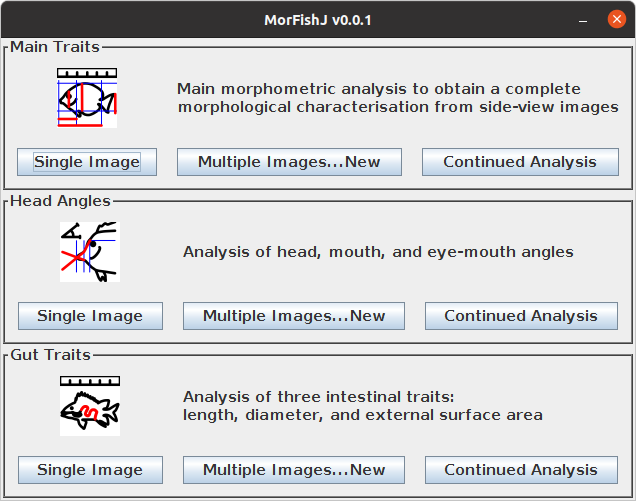
\includegraphics[width=0.6\textwidth,height=\textheight]{./images/screenshots/MorFishJ_GUI_v0.0.1.png}

}

\end{figure}

\begin{tcolorbox}[standard jigsaw,arc=.35mm, toptitle=1mm, titlerule=0mm, bottomtitle=1mm, left=2mm, colbacktitle=quarto-callout-tip-color!10!white, colback=white, opacityback=0, leftrule=.75mm, title=\textcolor{quarto-callout-tip-color}{\faLightbulb}\hspace{0.5em}{Tip}, coltitle=black, rightrule=.15mm, bottomrule=.15mm, toprule=.15mm, opacitybacktitle=0.6, colframe=quarto-callout-tip-color-frame]
In Fiji the Plugins menu is often crowded, thus it may be easier to use
the \texttt{Search} field under the toolbar to find and start
\texttt{MorFishJ}.
\end{tcolorbox}

\hypertarget{gui}{%
\chapter{GUI}\label{gui}}

\begin{figure}

{\centering 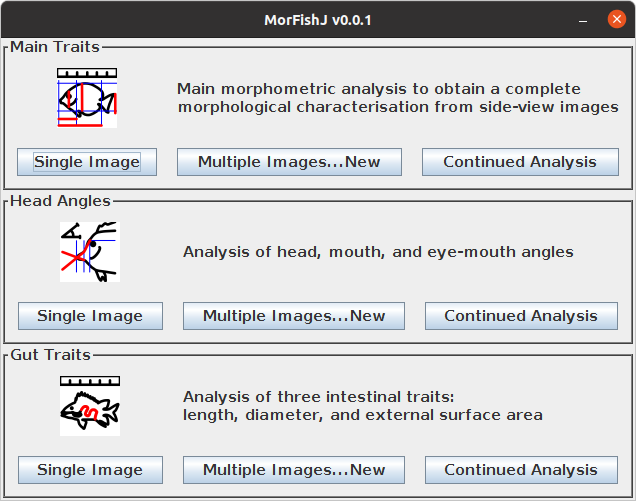
\includegraphics[width=0.7\textwidth,height=\textheight]{./images/screenshots/MorFishJ_GUI_v0.0.1.png}

}

\end{figure}

The GUI of \texttt{MorFishJ} provides a simple and direct access to all
the morphometric analyses. Each analysis can be started by clicking on
the appropriate button.

\hypertarget{morphometric-analyses}{%
\section{Morphometric analyses}\label{morphometric-analyses}}

Three morphometric analyses are currently available in
\texttt{MorFishJ}:

\begin{tcolorbox}[standard jigsaw,arc=.35mm, toptitle=1mm, titlerule=0mm, bottomtitle=1mm, left=2mm, colbacktitle=quarto-callout-note-color!10!white, colback=white, opacityback=0, leftrule=.75mm, title={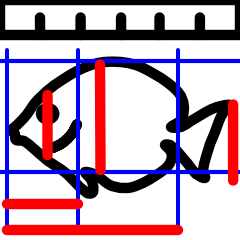
\includegraphics[width=0.3125in,height=\textheight]{./images/icons/FishTraitsIcon.png}
Main Traits}, coltitle=black, rightrule=.15mm, bottomrule=.15mm, toprule=.15mm, opacitybacktitle=0.6, colframe=quarto-callout-note-color-frame]
The workhorse of MorFishJ. Performs a complete morphometric analysis
measuring 22 traits that cover all body parts visible from side view
images, excluding dorsal, pelvic, and anal fins.
\end{tcolorbox}

\begin{tcolorbox}[standard jigsaw,arc=.35mm, toptitle=1mm, titlerule=0mm, bottomtitle=1mm, left=2mm, colbacktitle=quarto-callout-note-color!10!white, colback=white, opacityback=0, leftrule=.75mm, title={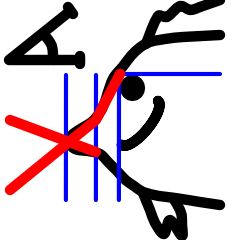
\includegraphics[width=0.3125in,height=\textheight]{./images/icons/HeadAnglesIcon.png}
Head Angles}, coltitle=black, rightrule=.15mm, bottomrule=.15mm, toprule=.15mm, opacitybacktitle=0.6, colframe=quarto-callout-note-color-frame]
It allows to measure three head angles related to vision and feeding
(Brandl and Bellwood 2013; Bellwood et al. 2014; Brandl, Robbins, and
Bellwood 2015).
\end{tcolorbox}

\begin{tcolorbox}[standard jigsaw,arc=.35mm, toptitle=1mm, titlerule=0mm, bottomtitle=1mm, left=2mm, colbacktitle=quarto-callout-note-color!10!white, colback=white, opacityback=0, leftrule=.75mm, title={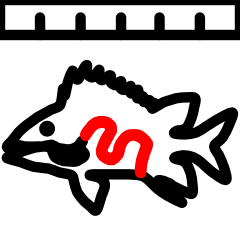
\includegraphics[width=0.3125in,height=\textheight]{./images/icons/GutTraitsIcon.png}
Gut Traits}, coltitle=black, rightrule=.15mm, bottomrule=.15mm, toprule=.15mm, opacitybacktitle=0.6, colframe=quarto-callout-note-color-frame]
It allows to measure three intestinal traits related to fish diet
(Ghilardi et al. 2021).
\end{tcolorbox}

\hypertarget{sec-setup}{%
\section{Single and multiple image analysis}\label{sec-setup}}

Each analysis has three different buttons:

\begin{itemize}
\tightlist
\item
  \textbf{Single Image}: to analyse only one image (may be useful for
  beginners to get used to each step before analysing the entire image
  database).
\item
  \textbf{Multiple Images\ldots New}: to start a new analysis of an
  image database.
\item
  \textbf{Continued Analysis}: to continue analysing an image database
  from where it was last left.
\end{itemize}

\hypertarget{single-image}{%
\subsection{Single Image}\label{single-image}}

\begin{tcolorbox}[standard jigsaw,arc=.35mm, toptitle=1mm, titlerule=0mm, bottomtitle=1mm, left=2mm, colbacktitle=quarto-callout-warning-color!10!white, colback=white, opacityback=0, leftrule=.75mm, title=\textcolor{quarto-callout-warning-color}{\faExclamationTriangle}\hspace{0.5em}{Warning}, coltitle=black, rightrule=.15mm, bottomrule=.15mm, toprule=.15mm, opacitybacktitle=0.6, colframe=quarto-callout-warning-color-frame]
An image must be opened before starting a single image analysis.
\end{tcolorbox}

Clicking on the \texttt{Single\ Image} button of the desired analysis
before opening an image will display the following message.

\begin{figure}

{\centering 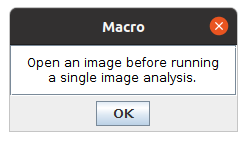
\includegraphics[width=0.3\textwidth,height=\textheight]{./images/screenshots/single_image_error.png}

}

\end{figure}

To open an image click on \textbf{File --\textgreater{} Open\ldots{}} or
use the shortcut \textbf{Ctrl+O} or drag the image over the ImageJ GUI.

Once the image is opened click on the \texttt{Single\ Image} button of
the desired analysis. The image is duplicated and all the following
steps will be performed on the duplicated image to avoid any unwanted
modification of the raw image. The \texttt{ROI\ Manager} window is
automatically opened and the first dialog box appears, to either set the
scale or adjust the image, depending on the type of analysis selected.

The steps required to perform the selected analysis are explained in the
following chapters.

\hypertarget{multiple-images}{%
\subsection{Multiple Images}\label{multiple-images}}

\hypertarget{new-analysis}{%
\subsubsection*{New analysis}\label{new-analysis}}
\addcontentsline{toc}{subsubsection}{New analysis}

Before starting to analyse an image database the new project should have
a clear folder structure. \texttt{MorFishJ} does not require a fixed
folder structure, but only an input directory where the raw images are
stored and two output directories, one to save the ROIs and one to save
the results and log files (although the same output directory could be
used for all outputs). Therefore, you can set your own folder structure.
However, it is advisable that each project has its own directory with
the following structure.

\begin{verbatim}
./ProjectName/
├── raw_images
│   ├── img1.JPG
│   ├── img2.JPG
│   ├── img3.JPG
│   └── ...
├── results
└── ROIs
\end{verbatim}

There are three subdirectories: one containing the raw images, one to
save the ROIs and processed images, and one to save the results and log
files.

To start a new analysis click on the \texttt{Multiple\ Images...New}
button of the desired analysis. The following dialog box appears.

\begin{figure}

{\centering 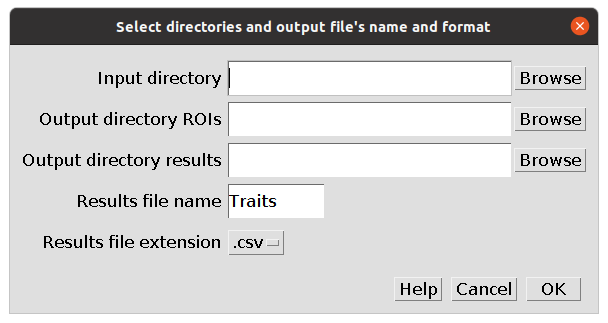
\includegraphics[width=0.7\textwidth,height=\textheight]{./images/screenshots/dialog_select_directories.png}

}

\end{figure}

Use the \texttt{Browse} button to add the path to the input directory
where the raw images are stored, and the output directories where the
ROIs and results will be saved. Alternatively, it is possible to drag
the directories over the dialog box. By default the results file will be
named \textbf{Traits} and will be saved in \texttt{.csv} format, but it
is possible to change both the name and the extension, which can be
changed to \texttt{.txt} through the drop-down list.

Once all the fields are completed click \texttt{OK}. Two files are
created in the selected directory for the results:

\begin{itemize}
\tightlist
\item
  a log file with the name \texttt{TraitLog} followed by the date of
  creation in \texttt{dd\_mm\_yyyy} format and including all the
  metadata required to restore the project.
\item
  a results file with the selected name and extension. Results are
  appended to this file at the completion of the analysis of each image.
\end{itemize}

\begin{tcolorbox}[standard jigsaw,arc=.35mm, toptitle=1mm, titlerule=0mm, bottomtitle=1mm, left=2mm, colbacktitle=quarto-callout-important-color!10!white, colback=white, opacityback=0, leftrule=.75mm, title=\textcolor{quarto-callout-important-color}{\faExclamation}\hspace{0.5em}{Important}, coltitle=black, rightrule=.15mm, bottomrule=.15mm, toprule=.15mm, opacitybacktitle=0.6, colframe=quarto-callout-important-color-frame]
Do not edit the \texttt{TraitLog} file by hand and do not change its
directory!
\end{tcolorbox}

The first image in the input directory is automatically opened and
duplicated. All the following steps will be performed on the duplicated
image to avoid any unwanted modification of the raw image. The
\texttt{ROI\ Manager} window is automatically opened and the first
dialog box appears, to either set the scale or adjust the image,
depending on the type of analysis selected.

The steps required to perform the selected analysis are explained in:

\begin{itemize}
\tightlist
\item
  Chapter~\ref{sec-main_traits}: \textbf{Main Traits}
\item
  Chapter~\ref{sec-head_angles}: \textbf{Head Angles}
\item
  \textbf{?@sec-gut\_traits}: \textbf{Gut Traits}
\end{itemize}

\hypertarget{continued-analysis}{%
\subsubsection*{Continued analysis}\label{continued-analysis}}
\addcontentsline{toc}{subsubsection}{Continued analysis}

It is possible to stop and restart each analysis without losing
progress. Everything done until the last completed image is saved, thus,
if the analysis is stopped before completing an image, only the steps
performed on that image are lost.

To continue a project from where it was last left, click on the
\texttt{Continued\ Analysis} button of the desired analysis. The
following dialog box appears.

\begin{figure}

{\centering 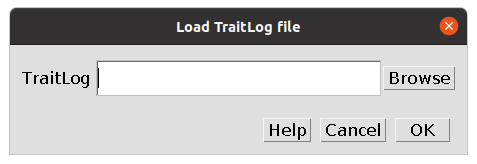
\includegraphics[width=0.6\textwidth,height=\textheight]{./images/screenshots/load_traitlog.png}

}

\end{figure}

Use the \texttt{Browse} button or drag the file over the dialog box to
add the path to the \texttt{TraitLog} file of the project. Thus click
\texttt{OK}. The project is restored and can be continued from the next
image. The new results will be appended to the existing results file.

\hypertarget{sec-set_scale}{%
\chapter{Set scale}\label{sec-set_scale}}

Two analyses, \texttt{Main\ Traits} and \texttt{Gut\ Traits}, require to
set the scale for the image. This is the first step of both analyses.
The following dialog box appears.

\begin{figure}

{\centering 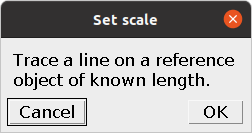
\includegraphics[width=0.3\textwidth,height=\textheight]{./images/screenshots/set_scale_info.png}

}

\end{figure}

Trace a straight line on a reference object and click \texttt{OK}.

\begin{tcolorbox}[standard jigsaw,arc=.35mm, toptitle=1mm, titlerule=0mm, bottomtitle=1mm, left=2mm, colbacktitle=quarto-callout-tip-color!10!white, colback=white, opacityback=0, leftrule=.75mm, title=\textcolor{quarto-callout-tip-color}{\faLightbulb}\hspace{0.5em}{Tip}, coltitle=black, rightrule=.15mm, bottomrule=.15mm, toprule=.15mm, opacitybacktitle=0.6, colframe=quarto-callout-tip-color-frame]
The reference object can also be the fish itself if its length
(standard, fork, or total) is known. In this case trace a line over the
fish to select the appropriate length.
\end{tcolorbox}

The following dialog box appears.

\begin{figure}

{\centering 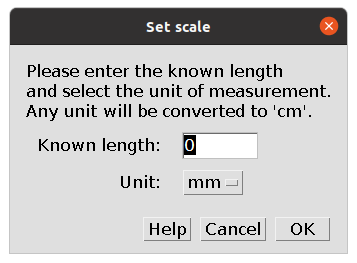
\includegraphics[width=0.4\textwidth,height=\textheight]{./images/screenshots/set_scale_dialog.png}

}

\end{figure}

Enter the known length of the traced line and select the unit from the
drop-down list. Three options are available (\emph{mm}, \emph{cm}, and
\emph{inch}), but any unit will then be converted to \emph{cm}. Thus all
linear measurements will be saved in \emph{cm} and areas in
\emph{cm\textsuperscript{2}}.

The traced line will be stored in the ROI Manager as \texttt{px.cm} and
then saved with all other ROIs. A column \texttt{px.cm} will also be
included in the results file indicating the scale of the images in
pixels/cm.

\begin{tcolorbox}[standard jigsaw,arc=.35mm, toptitle=1mm, titlerule=0mm, bottomtitle=1mm, left=2mm, colbacktitle=quarto-callout-warning-color!10!white, colback=white, opacityback=0, leftrule=.75mm, title=\textcolor{quarto-callout-warning-color}{\faExclamationTriangle}\hspace{0.5em}{Warning}, coltitle=black, rightrule=.15mm, bottomrule=.15mm, toprule=.15mm, opacitybacktitle=0.6, colframe=quarto-callout-warning-color-frame]
At the moment it is not possible to run the \texttt{Main\ Traits} and
\texttt{Gut\ Traits} analyses on images without a reference object or
known fish length as setting the scale is required. However, in the
upcoming update setting the scale will become optional and all images
can be analysed.
\end{tcolorbox}

\hypertarget{sec-straighten_rotate}{%
\chapter{Straighten and rotate}\label{sec-straighten_rotate}}

Two analyses, \texttt{Main\ Traits} and \texttt{Head\ Angles}, require
the fish to be in a straight and horizontal position. For such analyses
the software allows to adjust the image if required. For the
\texttt{Main\ Traits} analysis this is the second step, after setting
the scale (as described in Chapter~\ref{sec-set_scale}), whereas for the
\texttt{Head\ Angles} analysis it is the first step. The following
dialog box appears.

\begin{figure}

{\centering 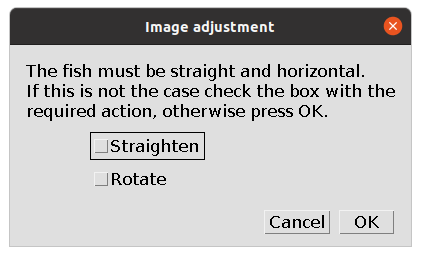
\includegraphics[width=0.5\textwidth,height=\textheight]{./images/screenshots/adjust_image.png}

}

\end{figure}

It allows to select one of two options:

\begin{itemize}
\tightlist
\item
  \texttt{Straighten}: to straighten the fish if it is in a bent
  position.
\item
  \texttt{Rotate}: to rotate the image and set the fish in an horizontal
  position.
\end{itemize}

Therefore, if the fish is not straight and horizontal, select the
appropriate option and click \texttt{OK}. Otherwise, click \texttt{OK}
without selecting any option and continue.

\hypertarget{straighten}{%
\section*{Straighten}\label{straighten}}
\addcontentsline{toc}{section}{Straighten}

When the fish is bent, select \texttt{Straighten} and click \texttt{OK}.
The following dialog box appears together with the \texttt{Line\ Width}
window.

\begin{figure}

{\centering 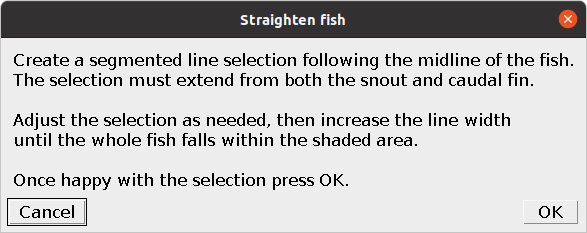
\includegraphics[width=0.7\textwidth,height=\textheight]{./images/screenshots/straighten_dialog.png}

}

\end{figure}

Follow the instructions given in the dialog box, create a segmented line
selection, adjust the width and click \texttt{OK}. The fish will be
straightened and in an horizontal position. The following figure shows
an example of fish straightening.

\hypertarget{before}{%
\subsubsection{\texorpdfstring{\textbf{Before}}{Before}}\label{before}}

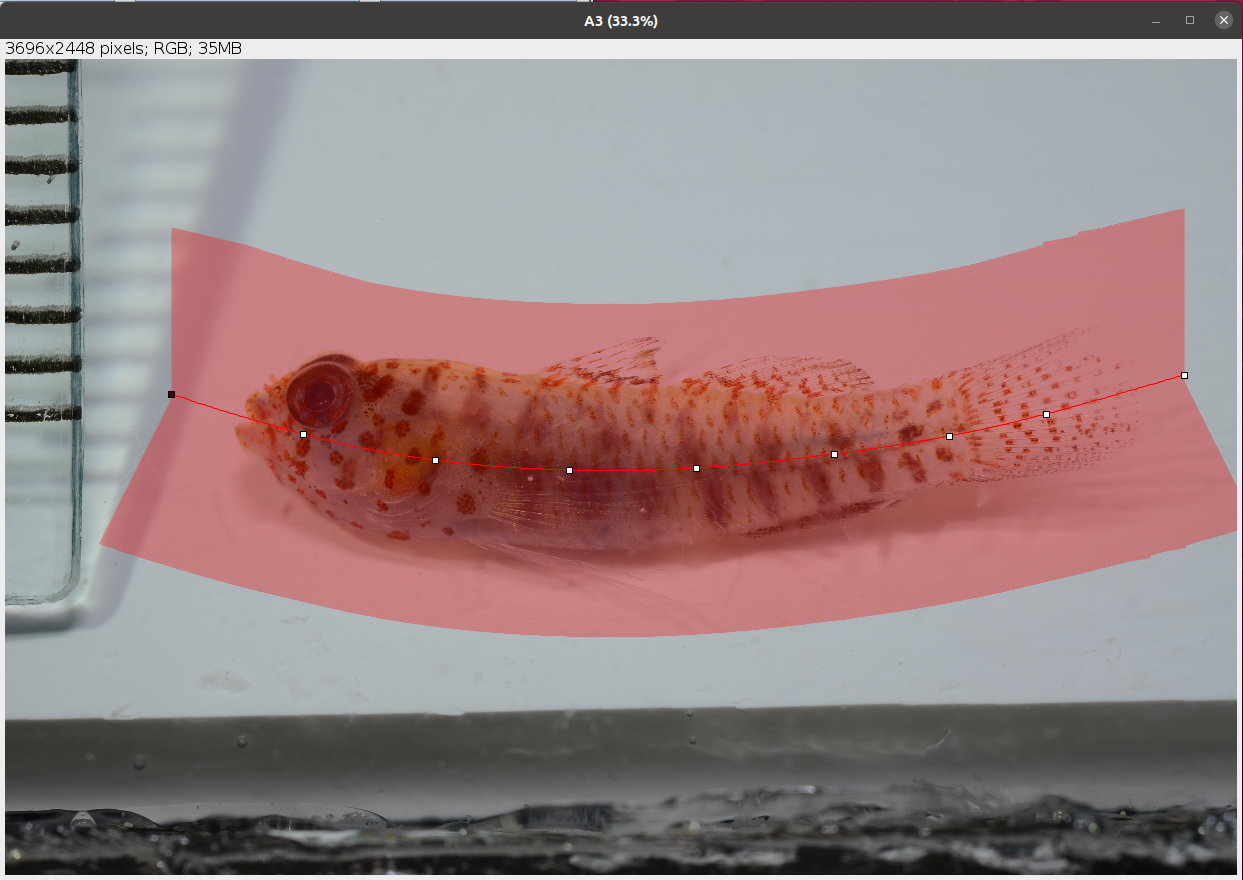
\includegraphics{./images/screenshots/straighten_example.png}

\hypertarget{after}{%
\subsubsection{\texorpdfstring{\textbf{After}}{After}}\label{after}}

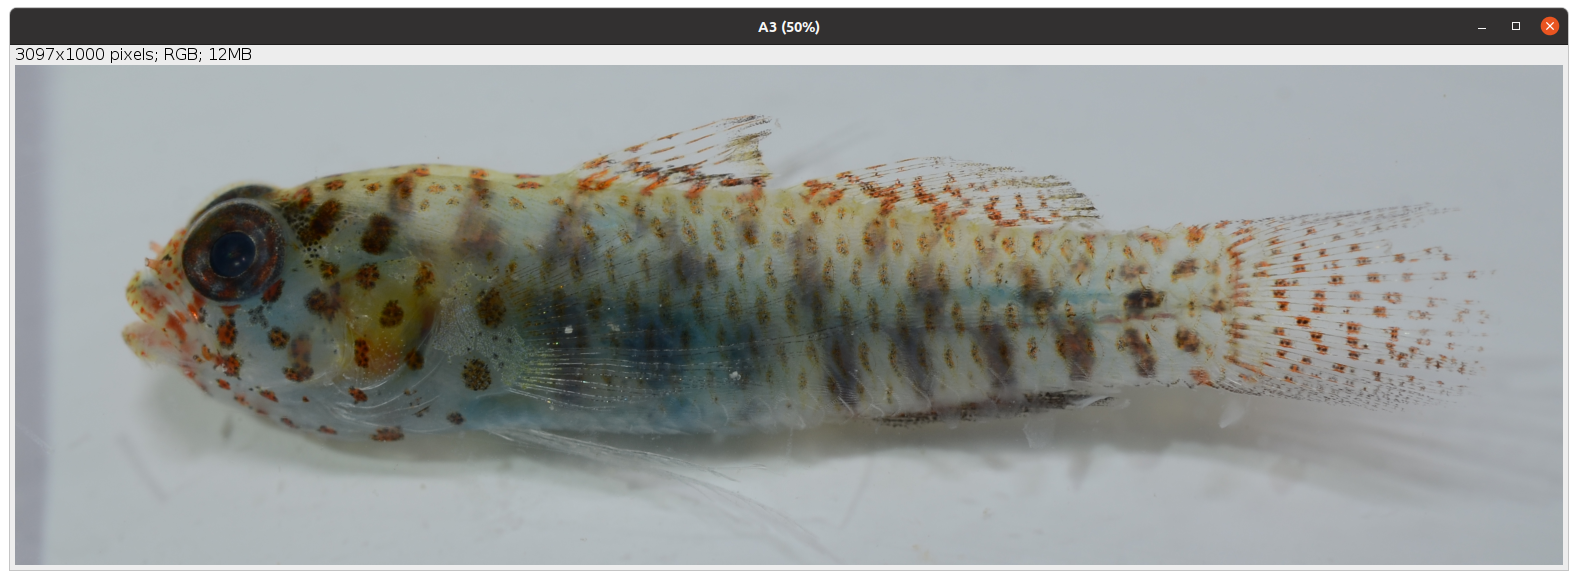
\includegraphics{./images/screenshots/straightened_example.png}

\begin{tcolorbox}[standard jigsaw,arc=.35mm, toptitle=1mm, titlerule=0mm, bottomtitle=1mm, left=2mm, colbacktitle=quarto-callout-tip-color!10!white, colback=white, opacityback=0, leftrule=.75mm, title=\textcolor{quarto-callout-tip-color}{\faLightbulb}\hspace{0.5em}{Tip}, coltitle=black, rightrule=.15mm, bottomrule=.15mm, toprule=.15mm, opacitybacktitle=0.6, colframe=quarto-callout-tip-color-frame]
Selecting \texttt{Spline\ fit} within the \texttt{Line\ Width} window
can improve the selection and straightening of the fish.
\end{tcolorbox}

\begin{tcolorbox}[standard jigsaw,arc=.35mm, toptitle=1mm, titlerule=0mm, bottomtitle=1mm, left=2mm, colbacktitle=quarto-callout-warning-color!10!white, colback=white, opacityback=0, leftrule=.75mm, title=\textcolor{quarto-callout-warning-color}{\faExclamationTriangle}\hspace{0.5em}{Warning}, coltitle=black, rightrule=.15mm, bottomrule=.15mm, toprule=.15mm, opacitybacktitle=0.6, colframe=quarto-callout-warning-color-frame]
If the fish is overly bent, straightening can lead to deformation of the
body which affects the measurement of the traits. Use this option with
care.
\end{tcolorbox}

\hypertarget{rotate}{%
\section*{Rotate}\label{rotate}}
\addcontentsline{toc}{section}{Rotate}

When the fish is straight but not horizontal, select \texttt{Rotate} and
click \texttt{OK}. The following dialog box appears.

\begin{figure}

{\centering 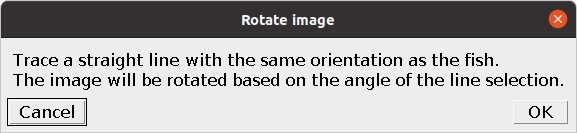
\includegraphics[width=0.7\textwidth,height=\textheight]{./images/screenshots/rotate_dialog.png}

}

\end{figure}

Follow the instructions given in the dialog box, trace a line and click
\texttt{OK}. The image will be rotated and, if the line was placed well,
the fish will be in an horizontal position. The following figure shows
an example of image rotation.

\hypertarget{before-1}{%
\subsubsection{\texorpdfstring{\textbf{Before}}{Before}}\label{before-1}}

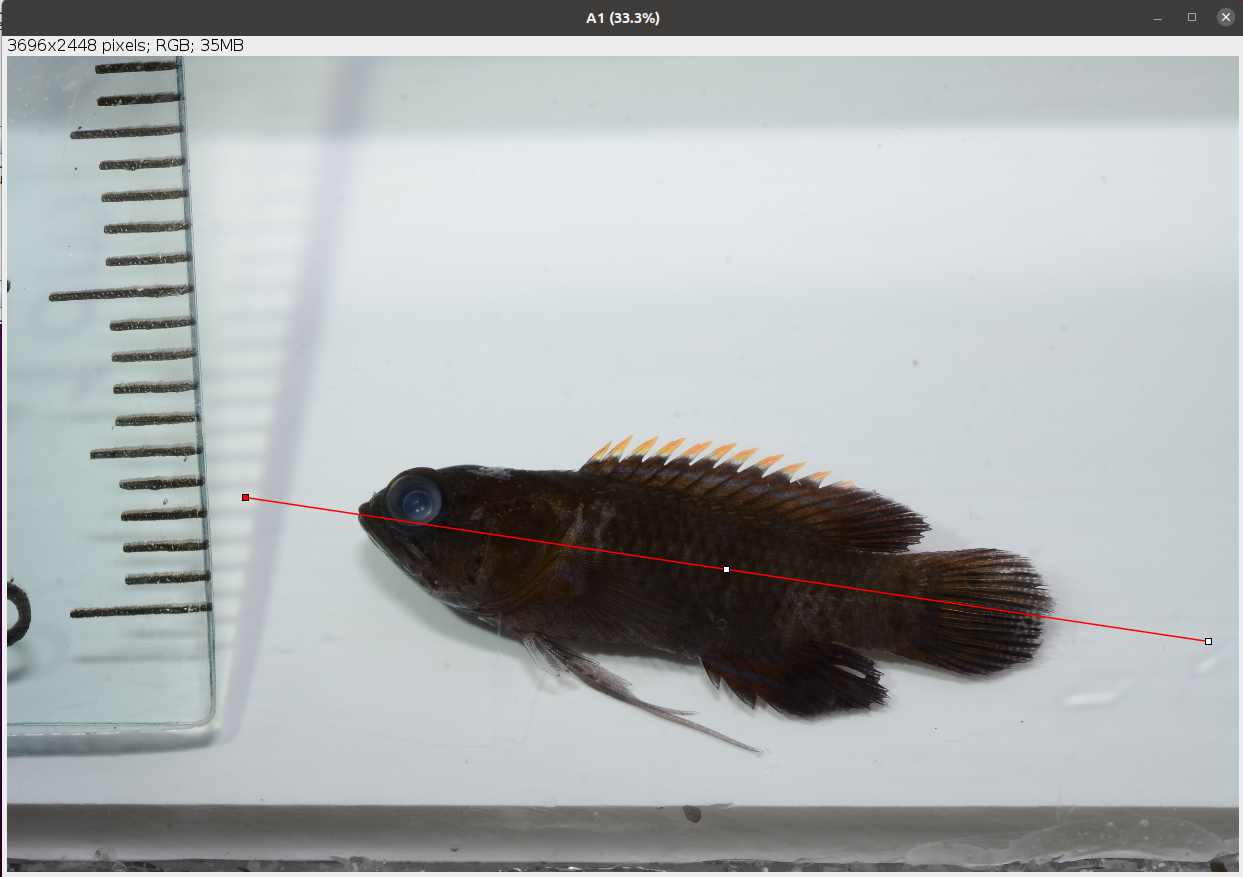
\includegraphics{./images/screenshots/rotate_example.png}

\hypertarget{after-1}{%
\subsubsection{\texorpdfstring{\textbf{After}}{After}}\label{after-1}}

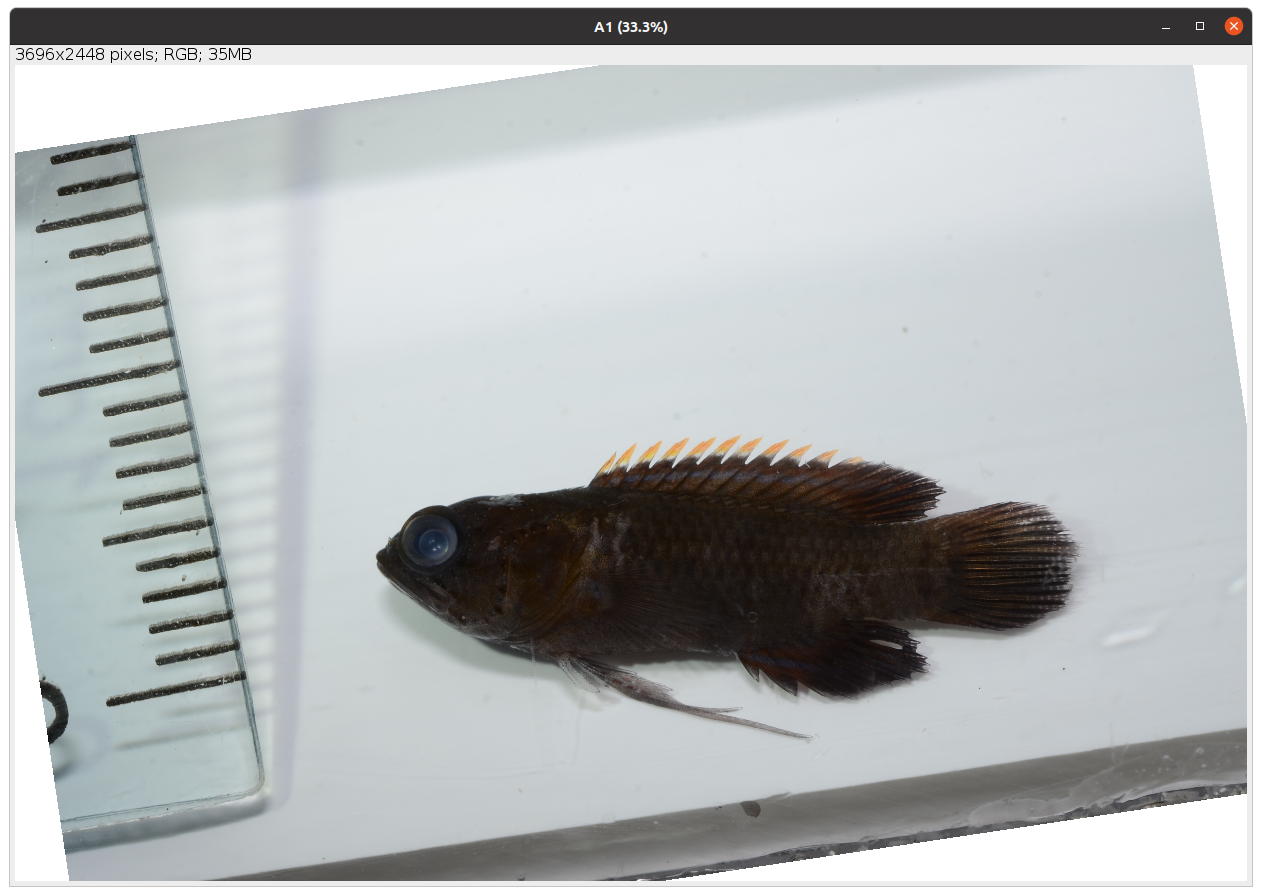
\includegraphics{./images/screenshots/rotated_example.png}

\hypertarget{sec-main_traits}{%
\chapter{Main Traits}\label{sec-main_traits}}

The \texttt{Main\ Traits} analysis is the workhorse of \texttt{MorFishJ}
as it performs a complete morphometric characterisation of fishes. It
requires the user input to trace the outline of the body and pectoral
fin, and to position some reference lines
(Figure~\ref{fig-main-ref-lines}, Table~\ref{tbl-main-ref-lines}) and
landmark points. The coordinates of these lines and points allow to
extract 22 morphometric measurements described in
Figure~\ref{fig-main-traits} and Table~\ref{tbl-main-traits-def}.

\begin{figure}

{\centering 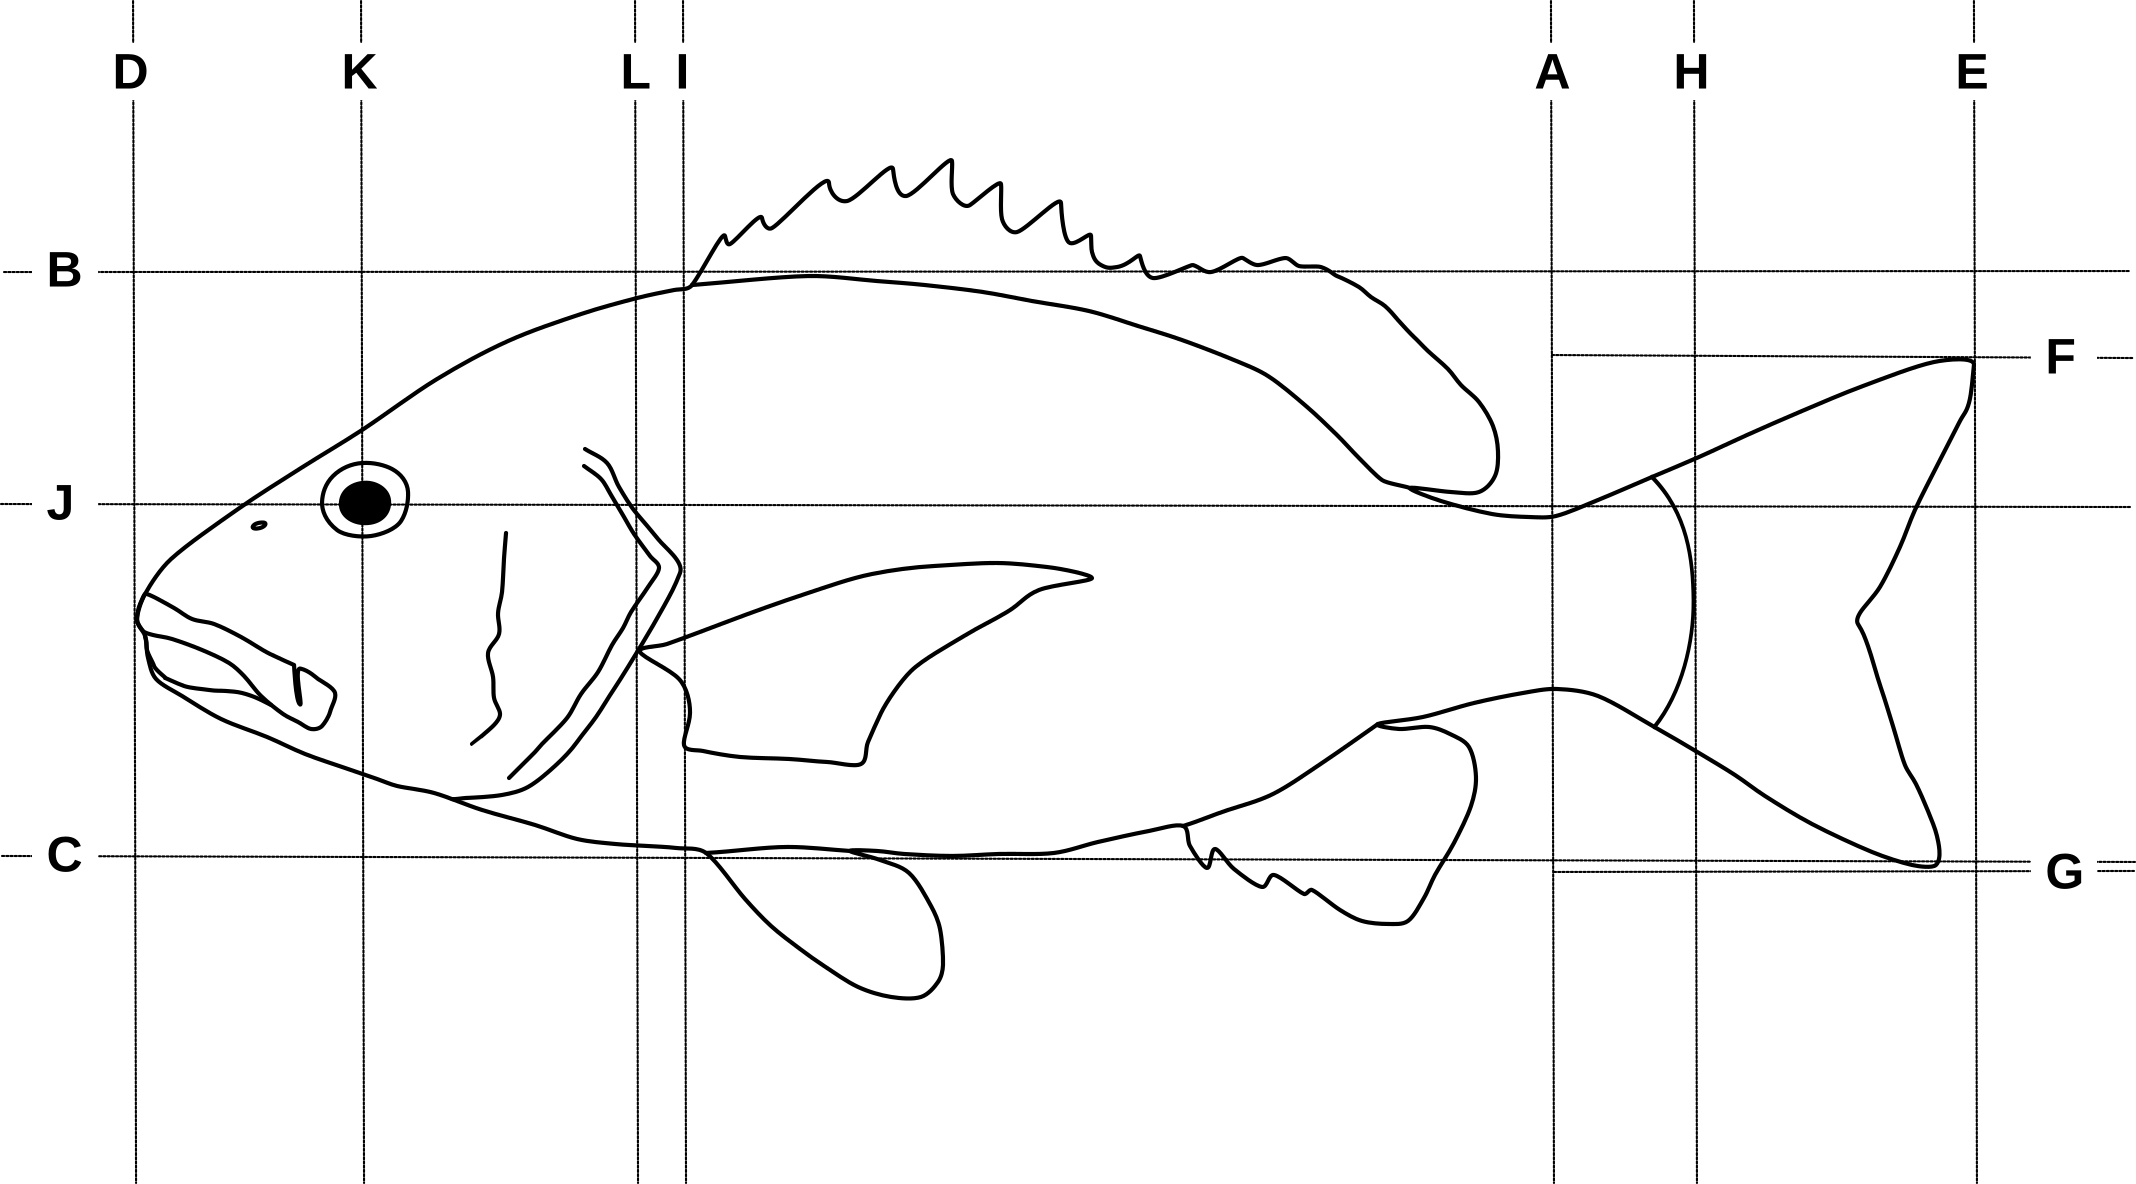
\includegraphics[width=0.8\textwidth,height=\textheight]{./images/drawings/main_ref_lines_sketch.png}

}

\caption{\label{fig-main-ref-lines}Reference lines traced on fish images
for main traits analysis (see Table~\ref{tbl-main-ref-lines} for
descriptions)}

\end{figure}

\begin{figure*}

\hypertarget{tbl-main-ref-lines}{}
\begin{longtable}[]{@{}
  >{\raggedright\arraybackslash}p{(\columnwidth - 4\tabcolsep) * \real{0.1781}}
  >{\raggedright\arraybackslash}p{(\columnwidth - 4\tabcolsep) * \real{0.6438}}
  >{\raggedright\arraybackslash}p{(\columnwidth - 4\tabcolsep) * \real{0.1781}}@{}}
\caption{\label{tbl-main-ref-lines}Description of reference lines traced
on fish images for main traits analysis}\tabularnewline
\toprule()
\begin{minipage}[b]{\linewidth}\raggedright
Reference line
\end{minipage} & \begin{minipage}[b]{\linewidth}\raggedright
Description
\end{minipage} & \begin{minipage}[b]{\linewidth}\raggedright
User input
\end{minipage} \\
\midrule()
\endfirsthead
\toprule()
\begin{minipage}[b]{\linewidth}\raggedright
Reference line
\end{minipage} & \begin{minipage}[b]{\linewidth}\raggedright
Description
\end{minipage} & \begin{minipage}[b]{\linewidth}\raggedright
User input
\end{minipage} \\
\midrule()
\endhead
A & Vertical line at the narrowest point of the caudal peduncle & Yes \\
B & Horizontal line touching the highest edge of the body (excluding
fins) & No \\
C & Horizontal line touching the lowest edge of the body (excluding
fins) & No \\
D & Vertical line touching the most anterior tip of the body & No \\
E & Vertical line touching the most posterior tip of the caudal fin &
No \\
F & Horizontal line touching the highest edge of the caudal fin & No \\
G & Horizontal line touching the lowest edge of the caudal fin & No \\
H & Vertical line at the base of the caudal fin (end of the vertebral
column or posterior edge of the hypural plate). Parrotfishes (Labridae:
Scarini) are an exception and the line should be placed between the last
and second to last scale lying along the midline
(\href{http://www.fishbase.us/glossary/Glossary.php?q=standard+length\&sc}{FishBase})
& Yes \\
I & Vertical line touching the posterior margin of the operculum &
Yes \\
J & Horizontal line cutting the eye in halves & Yes \\
K & Vertical line cutting the eye in halves & Yes \\
L & Vertical line at the pectoral fin insertion & Yes \\
\bottomrule()
\end{longtable}

\end{figure*}

\begin{figure}

\begin{minipage}[t]{0.10\linewidth}

{\centering 

~

}

\end{minipage}%
%
\begin{minipage}[t]{0.80\linewidth}

{\centering 

\raisebox{-\height}{

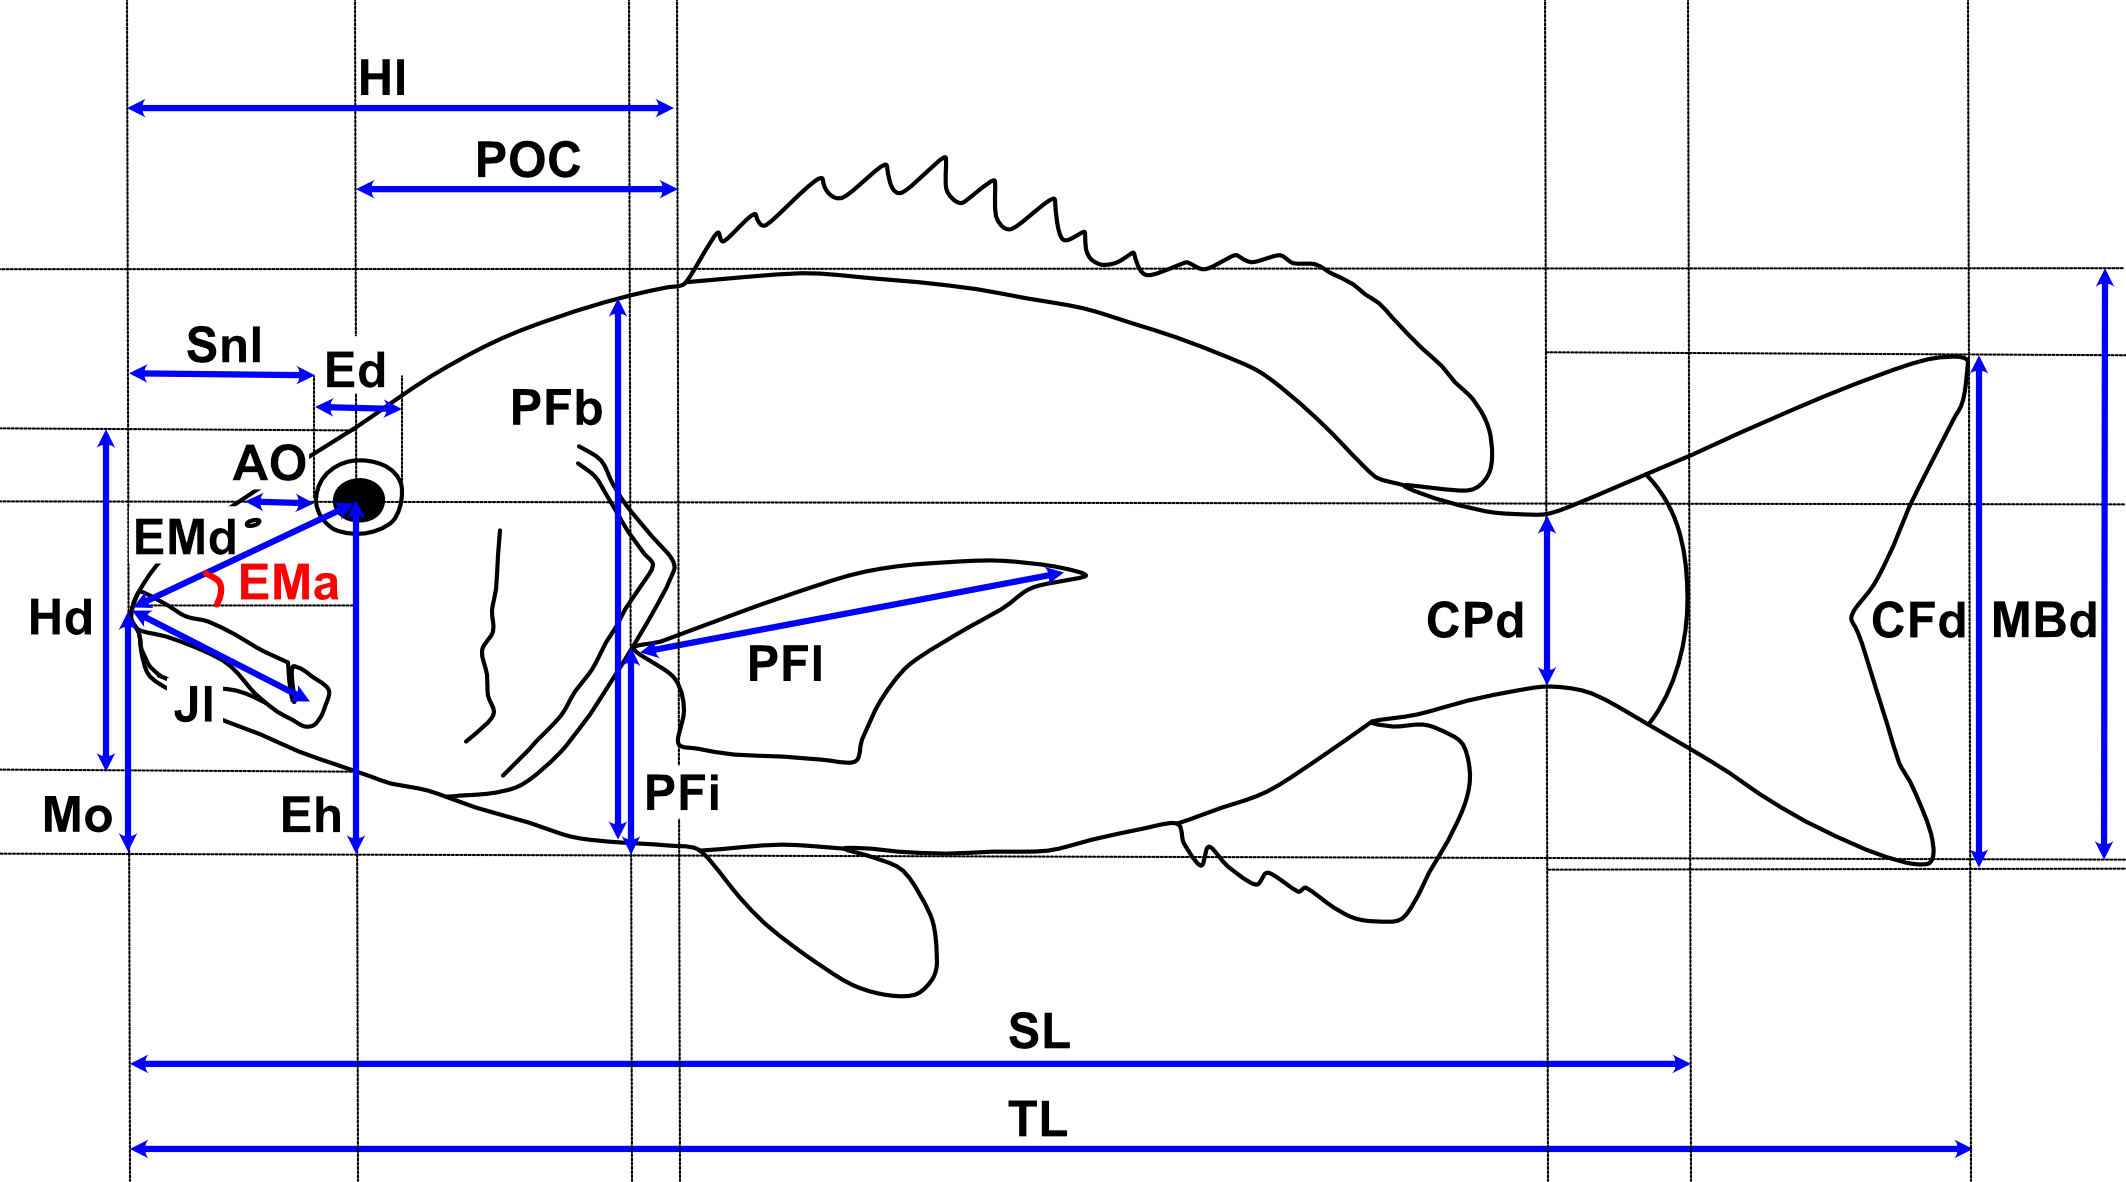
\includegraphics{./images/drawings/main_traits_sketch.png}

}

}

\subcaption{\label{fig-main-linear}Linear measurements}
\end{minipage}%
%
\begin{minipage}[t]{0.10\linewidth}

{\centering 

~

}

\end{minipage}%
\newline
\begin{minipage}[t]{0.10\linewidth}

{\centering 

~

}

\end{minipage}%
%
\begin{minipage}[t]{0.80\linewidth}

{\centering 

\raisebox{-\height}{

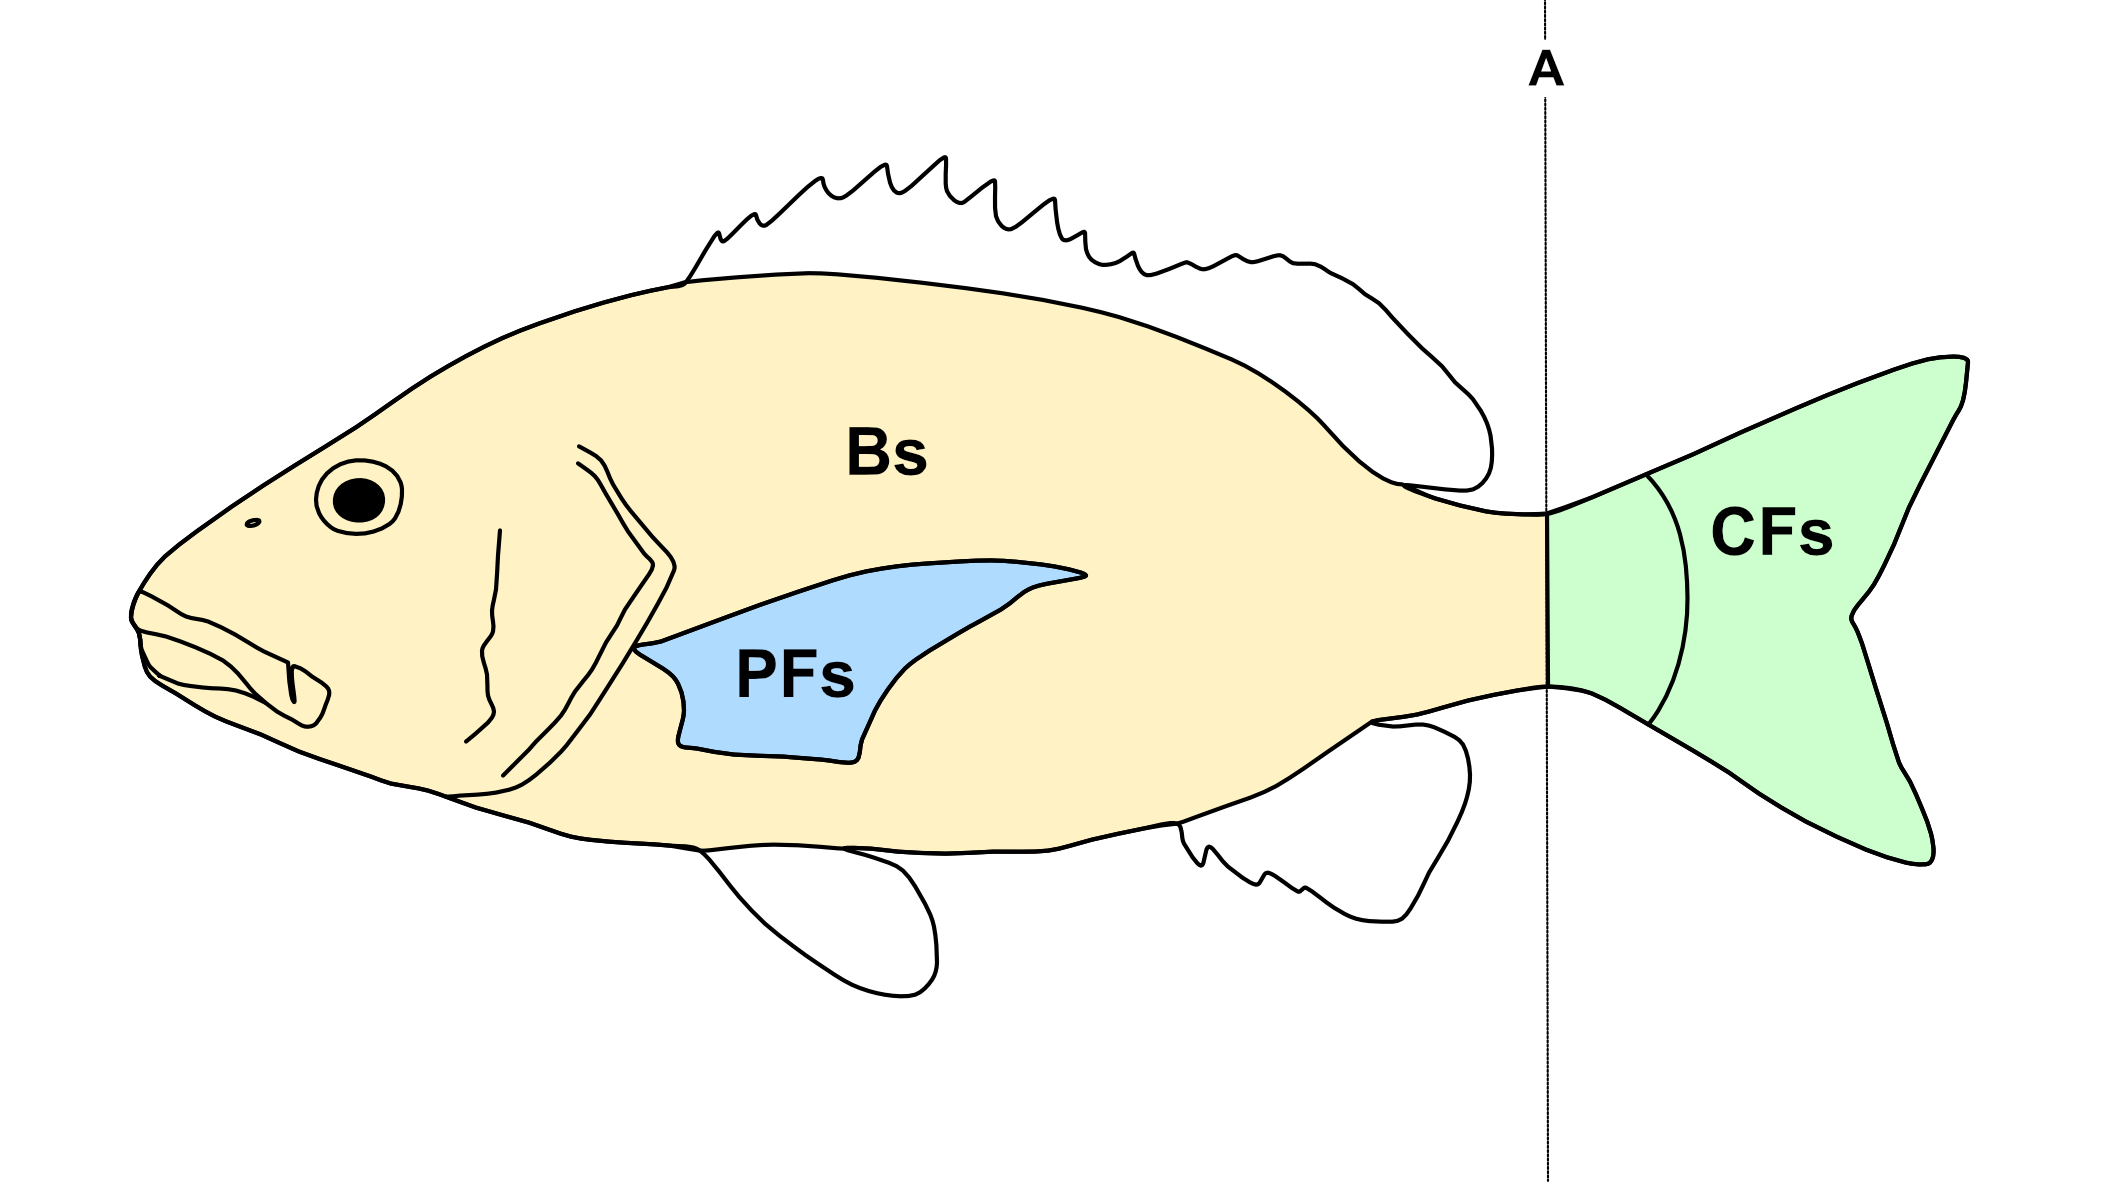
\includegraphics{./images/drawings/main_areas_sketch.png}

}

}

\subcaption{\label{fig-main-areas}Surface areas}
\end{minipage}%
%
\begin{minipage}[t]{0.10\linewidth}

{\centering 

~

}

\end{minipage}%

\caption{\label{fig-main-traits}Morphometric parameters taken on fish
images (see Table~\ref{tbl-main-traits-def} for descriptions)}

\end{figure}

\begin{figure*}

\hypertarget{tbl-main-traits-def}{}
\begin{longtable}[]{@{}
  >{\raggedright\arraybackslash}p{(\columnwidth - 6\tabcolsep) * \real{0.2027}}
  >{\raggedright\arraybackslash}p{(\columnwidth - 6\tabcolsep) * \real{0.2027}}
  >{\raggedright\arraybackslash}p{(\columnwidth - 6\tabcolsep) * \real{0.3919}}
  >{\raggedright\arraybackslash}p{(\columnwidth - 6\tabcolsep) * \real{0.2027}}@{}}
\caption{\label{tbl-main-traits-def}Description of morphometric
parameters taken on fish images}\tabularnewline
\toprule()
\begin{minipage}[b]{\linewidth}\raggedright
Code
\end{minipage} & \begin{minipage}[b]{\linewidth}\raggedright
Trait
\end{minipage} & \begin{minipage}[b]{\linewidth}\raggedright
Description
\end{minipage} & \begin{minipage}[b]{\linewidth}\raggedright
Reference
\end{minipage} \\
\midrule()
\endfirsthead
\toprule()
\begin{minipage}[b]{\linewidth}\raggedright
Code
\end{minipage} & \begin{minipage}[b]{\linewidth}\raggedright
Trait
\end{minipage} & \begin{minipage}[b]{\linewidth}\raggedright
Description
\end{minipage} & \begin{minipage}[b]{\linewidth}\raggedright
Reference
\end{minipage} \\
\midrule()
\endhead
TL & Total length & Length from the most anterior point of the body (D)
to the most posterior point (E) (excluding the caudal filaments) &
\href{http://www.fishbase.us/glossary/Glossary.php?q=total+length\&sc=is}{FishBase} \\
SL & Standard length & Length from most anterior point of the body (D)
to the the base of the caudal fin (H) &
\href{http://www.fishbase.us/glossary/Glossary.php?q=standard+length\&sc=is}{FishBase} \\
MBd & Maximum body depth & Body depth at the deepest part of the body
(excluding fins). Measured as the vertical distance between B and C &
Bellwood et al. (2014) \\
Hl & Head length & Horizontal distance from most anterior tip of the
head (D) to the posterior margin of the operculum (I) & Barnett,
Bellwood, and Hoey (2006) \\
Hd & Head depth & Head depth measured at the vertical of the orbit
centroid along K & Villéger et al. (2010) \\
Ed & Eye diameter & Internal diameter of the orbit measured along J &
Bellwood et al. (2014) \\
Eh & Eye position & Vertical distance from the orbit centroid (J × K) to
the bottom of the body (K × C) & Toussaint et al. (2016) \\
Snl & Snout length & Horizontal distance from the anterior margin of the
orbit to the tip of the snout (D) & Barnett, Bellwood, and Hoey
(2006) \\
POC & Posterior of orbit centroid & Horizontal distance from the orbit
centroid (J × K) to the posterior margin of the operculum (J × I) &
Bellwood et al. (2014) \\
AO & Anterior of orbit & Horizontal distance from the anterior margin of
the orbit to the anterior margin of the body along J (AO may be close,
or equal to, zero in species with very anterior eyes) & Bellwood et al.
(2014) \\
EMd & Eye-mouth distance & Distance between the orbit centroid (J × K)
to the anterior tip of the premaxilla & Bellwood et al. (2014) \\
EMa & Eye-mouth angle & Angle between EMd and a horizontal line
intersecting the tip of the premaxilla & Bellwood et al. (2014) \\
Mo & Oral gape position & Vertical distance from the tip of the
premaxilla to the bottom of the body (C) & Toussaint et al. (2016) \\
Jl & Maxillary jaw length & Length from the tip of the premaxilla to the
intersection between the maxilla and the mandible (i.e.~the corner of
the mouth) & Toussaint et al. (2016) \\
Bs & Body surface area & Area of a polygon drawn following the contour
of the body excluding fins, and up to the narrowest point of the caudal
peduncle & Bellwood et al. (2014) \\
CPd & Caudal peduncle depth & Measured at the narrowest point of the
caudal peduncle along A & Villéger et al. (2010) \\
CFd & Caudal fin depth & Maximum depth of the caudal fin & Villéger et
al. (2010) \\
CFs & Caudal fin surface area & Area of a polygon drawn following the
contour of the caudal fin, with the anterior margin marked by a straight
vertical line through the narrowest point of the caudal peduncle &
Villéger et al. (2010) \\
PFs & Pectoral fin surface area & Area of a polygon drawn following the
contour of the pectoral fin & Villéger et al. (2010) \\
PFl & Pectoral fin length & Length of the longest ray of the pectoral
fin & Toussaint et al. (2016) \\
PFi & Pectoral fin position & Vertical distance from the upper insertion
of the pectoral fin to the bottom of the body (C) & Toussaint et al.
(2016) \\
PFb & Body depth at level of pectoral fin insertion & Body depth
measured along L & Villéger et al. (2010) \\
\bottomrule()
\end{longtable}

\end{figure*}

\hypertarget{analysis}{%
\section{Analysis}\label{analysis}}

Once the steps described in Section~\ref{sec-setup} are completed the
screen will be populated with a number of windows:

\begin{itemize}
\tightlist
\item
  the ImageJ/Fiji main window
\item
  the MorFishJ GUI
\item
  a fish image (this is a duplicate of the raw image to prevent any
  modification)
\item
  the ROI manager
\item
  the \texttt{Set\ scale} dialog
\end{itemize}

While the majority of the analysis is automated, there are a number of
steps that require the user input:

\begin{enumerate}
\def\labelenumi{\arabic{enumi}.}
\item
  Set the scale for the image as described in
  Chapter~\ref{sec-set_scale}.
\item
  Adjust the image if necessary as described in
  Chapter~\ref{sec-straighten_rotate}.
\item
  Select the orientation of the fish (i.e., whether the fish is facing
  left or right) from a drop-down list. This step is important for the
  correct automatic placement of some reference lines and points.
\end{enumerate}

\begin{figure}

{\centering 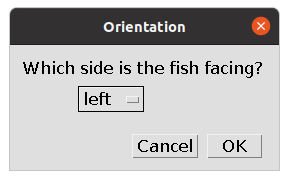
\includegraphics[width=0.3\textwidth,height=\textheight]{./images/screenshots/orientation.png}

}

\end{figure}

\begin{enumerate}
\def\labelenumi{\arabic{enumi}.}
\setcounter{enumi}{3}
\tightlist
\item
  Select the fish outline following the instruction in the dialog. Trace
  a polygon around the body and caudal fin, excluding the dorsal,
  pelvic, and anal fins as in the example below. Also avoid including
  any portion of pectoral fin protruding from the body area. Once the
  selection is completed it can be adjusted as needed.
\end{enumerate}

\begin{tcolorbox}[standard jigsaw,arc=.35mm, toptitle=1mm, titlerule=0mm, bottomtitle=1mm, left=2mm, colbacktitle=quarto-callout-tip-color!10!white, colback=white, opacityback=0, leftrule=.75mm, title=\textcolor{quarto-callout-tip-color}{\faLightbulb}\hspace{0.5em}{Tip}, coltitle=black, rightrule=.15mm, bottomrule=.15mm, toprule=.15mm, opacitybacktitle=0.6, colframe=quarto-callout-tip-color-frame]
The points that define the selection can be moved. To add a new point to
the selection press \texttt{Shift} and click on an existing point. To
remove one point press \texttt{Alt} and click on the point. See
\href{https://imagej.nih.gov/ij/docs/guide/146-19.html}{Polygon
Selection Tool}.
\end{tcolorbox}

\begin{figure}

{\centering 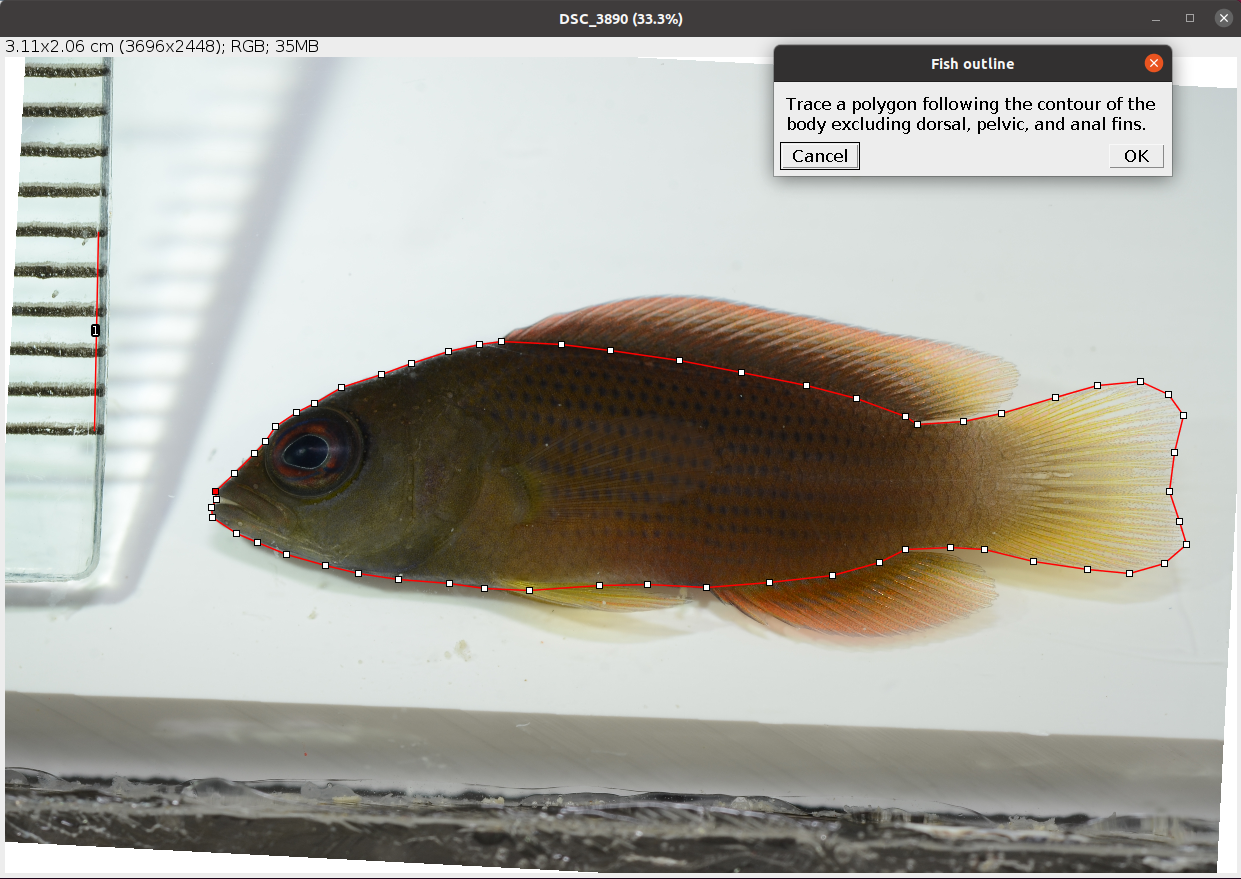
\includegraphics[width=0.8\textwidth,height=\textheight]{./images/screenshots/fish_outline.png}

}

\end{figure}

\begin{enumerate}
\def\labelenumi{\arabic{enumi}.}
\setcounter{enumi}{4}
\tightlist
\item
  Position reference line A at the narrowest point of the caudal
  peduncle. After clicking \texttt{OK} several automatic steps will
  split the outline in two, the body area (Bs) and caudal fin area
  (CFs), and add reference lines B-G.
\end{enumerate}

\begin{figure}

{\centering 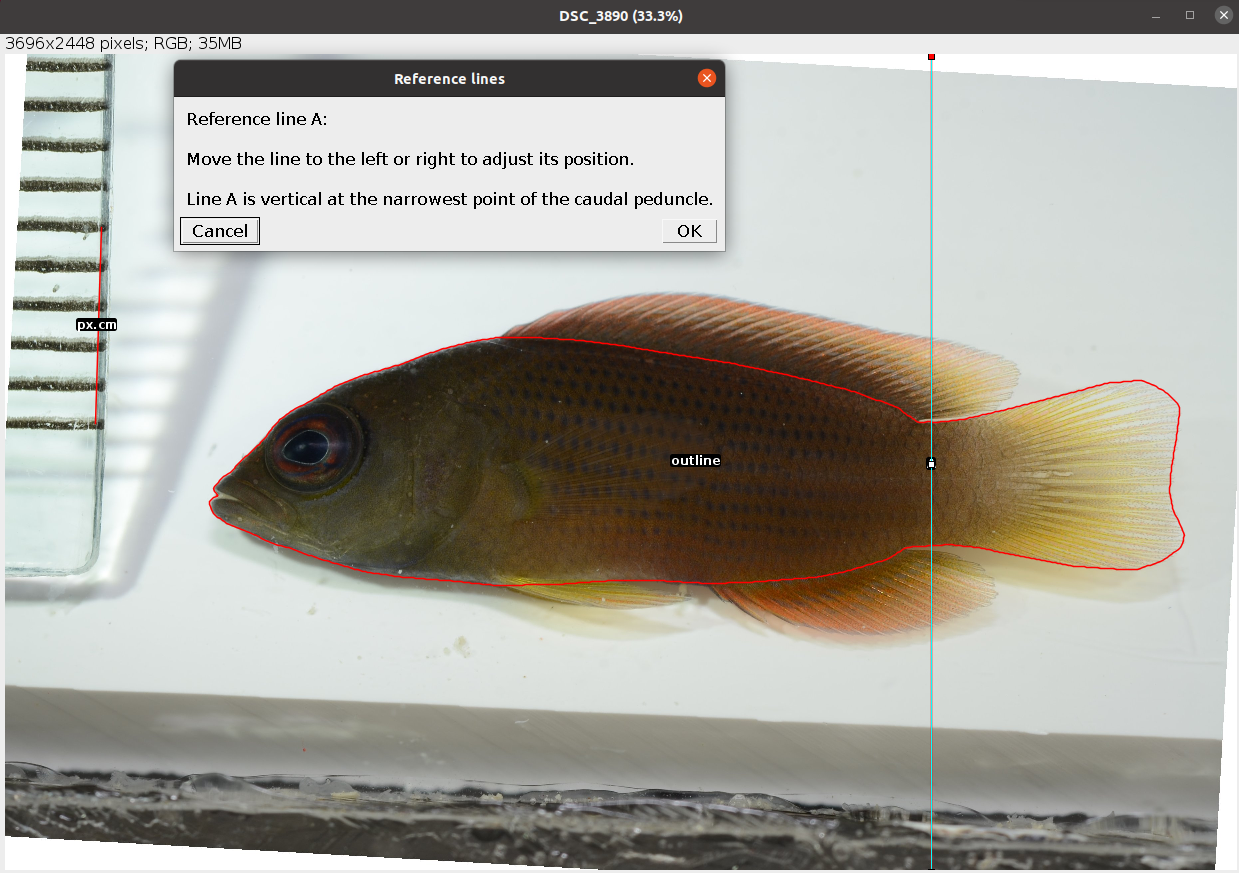
\includegraphics[width=0.8\textwidth,height=\textheight]{./images/screenshots/ref_lineA.png}

}

\end{figure}

\begin{enumerate}
\def\labelenumi{\arabic{enumi}.}
\setcounter{enumi}{5}
\tightlist
\item
  Position reference line H at the base of the caudal fin to mark the
  end of the standard length.
\end{enumerate}

\begin{figure}

{\centering 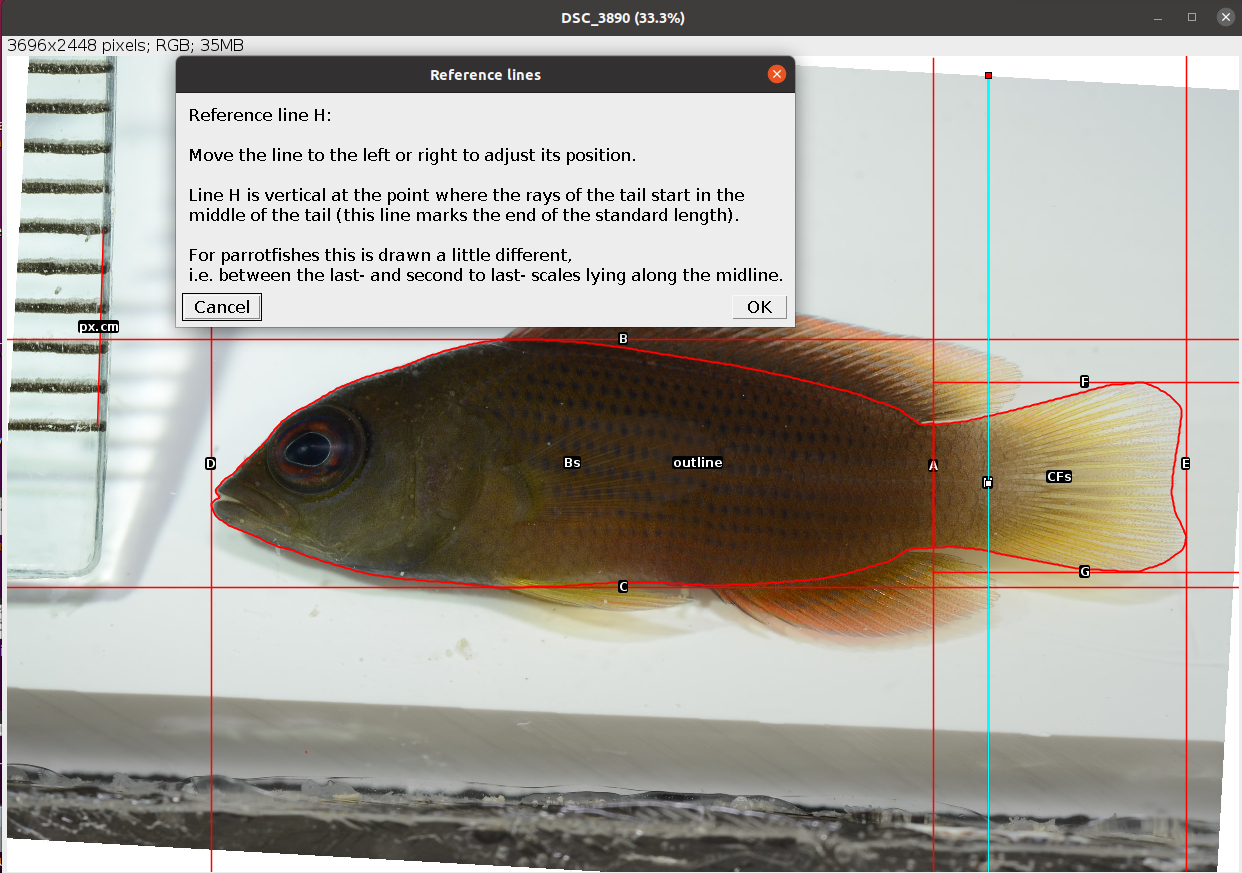
\includegraphics[width=0.8\textwidth,height=\textheight]{./images/screenshots/ref_lineH.png}

}

\end{figure}

\begin{enumerate}
\def\labelenumi{\arabic{enumi}.}
\setcounter{enumi}{6}
\tightlist
\item
  Position reference line I at the posterior margin of the operculum.
\end{enumerate}

\begin{figure}

{\centering 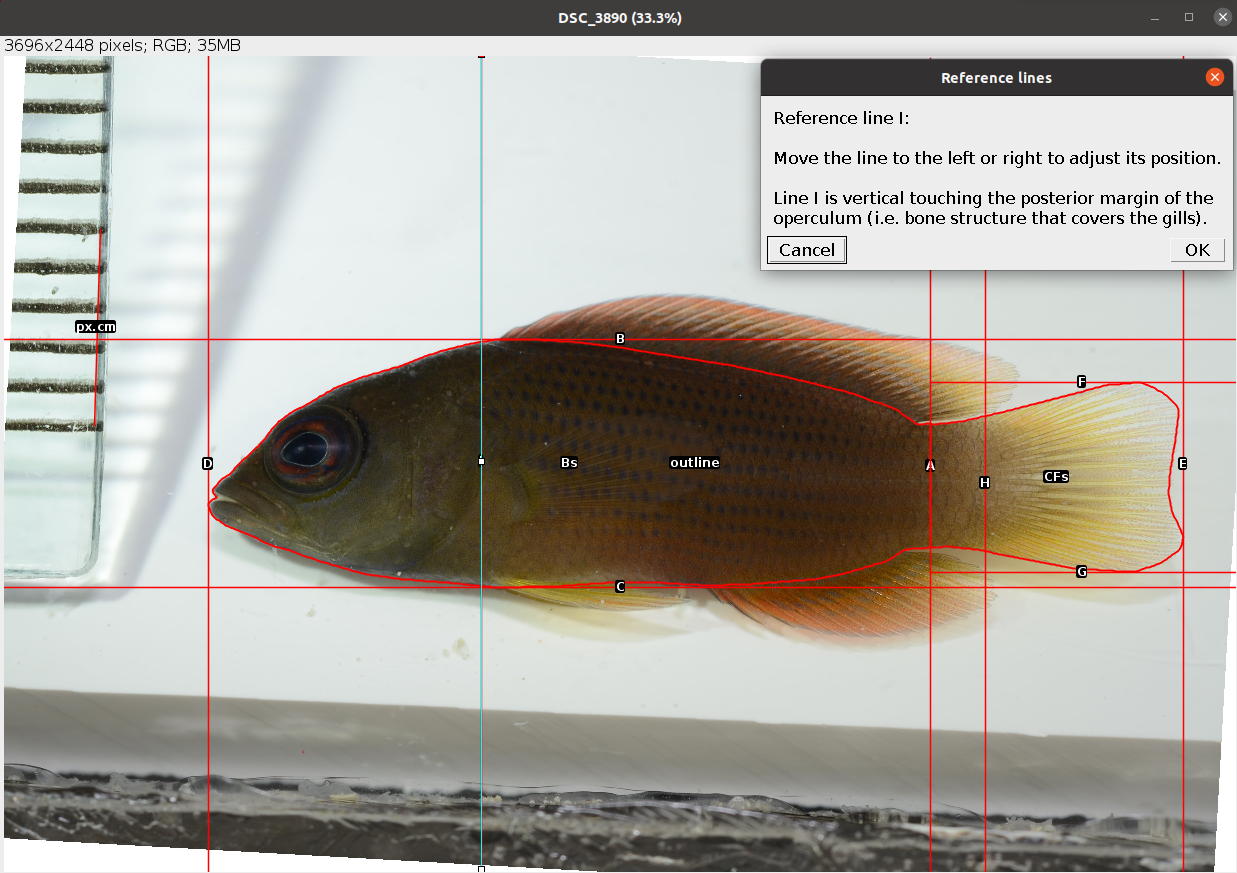
\includegraphics[width=0.8\textwidth,height=\textheight]{./images/screenshots/ref_lineI.png}

}

\end{figure}

\begin{enumerate}
\def\labelenumi{\arabic{enumi}.}
\setcounter{enumi}{7}
\tightlist
\item
  Trace an ellipse around the eye as in the example below (see
  \href{https://imagej.nih.gov/ij/docs/guide/146-19.html}{Elliptical
  Selection Tool} for specific instructions on how to use this tool).
  After clicking \texttt{OK} two new reference lines (J-K) are drawn
  perpendicular intersecting at the eye centroid.
\end{enumerate}

\begin{figure}

{\centering 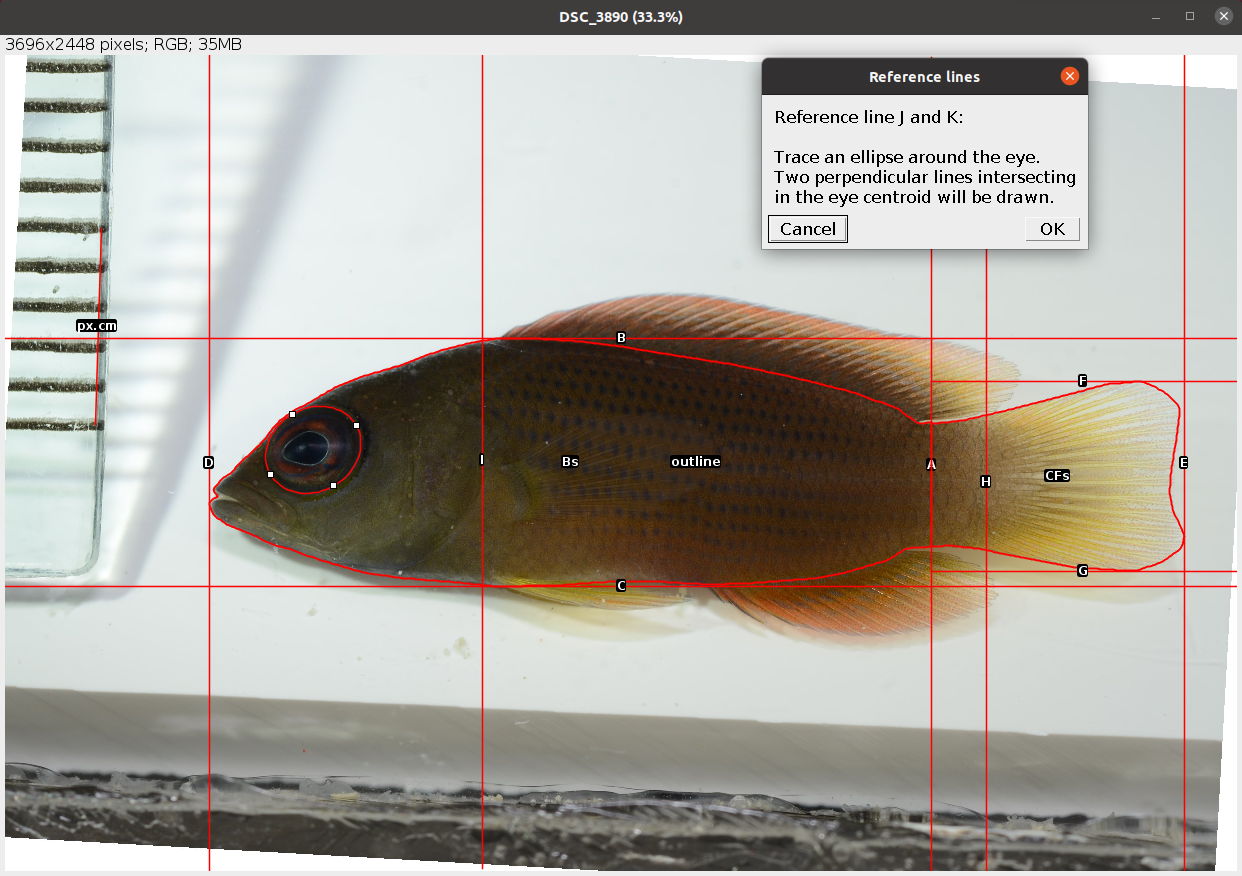
\includegraphics[width=0.8\textwidth,height=\textheight]{./images/screenshots/eye_ellipse.png}

}

\end{figure}

\begin{enumerate}
\def\labelenumi{\arabic{enumi}.}
\setcounter{enumi}{8}
\tightlist
\item
  Place a point at the insertion of the pectoral fin as in the example
  below.
\end{enumerate}

\begin{figure}

{\centering 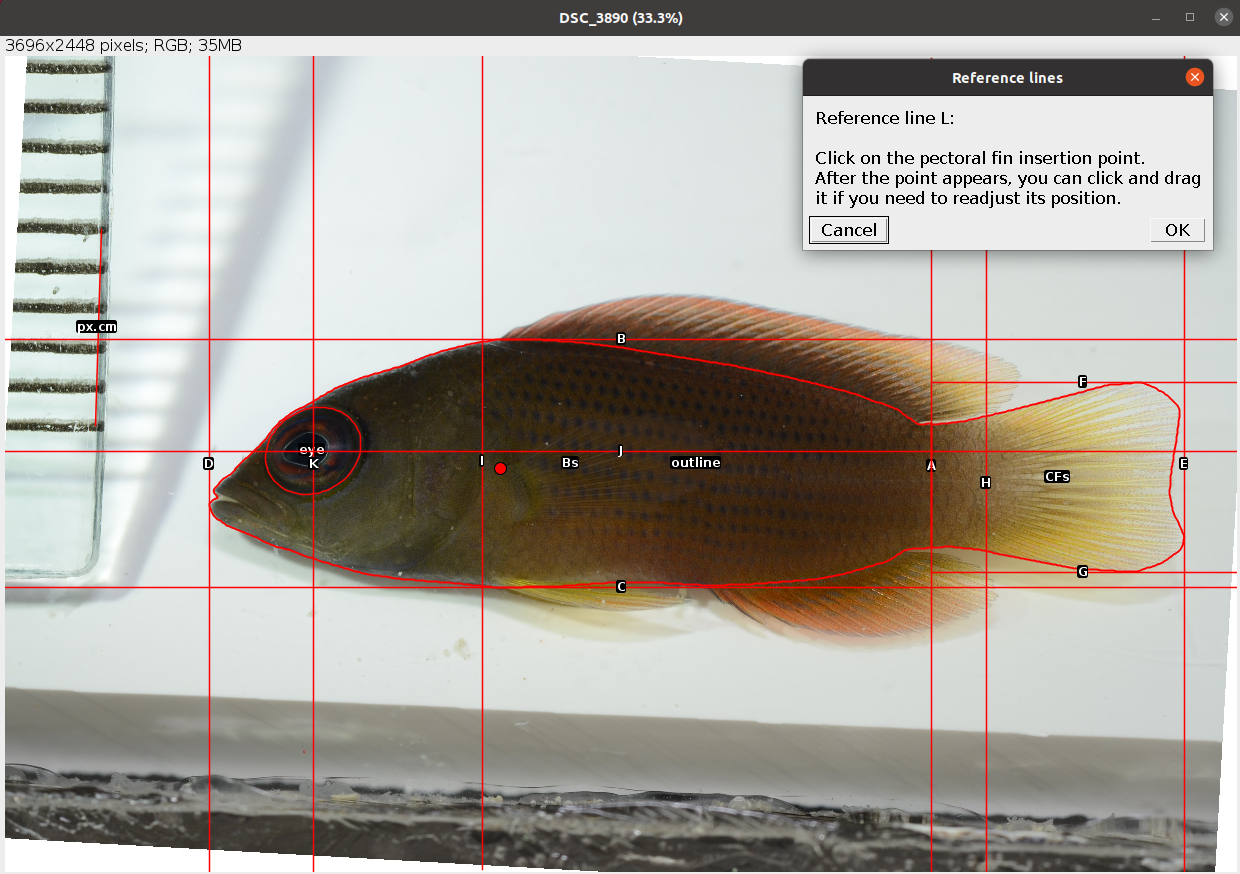
\includegraphics[width=0.8\textwidth,height=\textheight]{./images/screenshots/pectoral_fin_insertion.png}

}

\end{figure}

After clicking \texttt{OK} reference line L appears passing through the
selected point and 14 new traits are drawn and added to the ROI manager
together with all reference lines.

\begin{enumerate}
\def\labelenumi{\arabic{enumi}.}
\setcounter{enumi}{9}
\tightlist
\item
  Select the outline of the pectoral fin as in the example below. After
  clicking \texttt{OK} this is saved in the ROI manager as PFs.
\end{enumerate}

\begin{figure}

{\centering 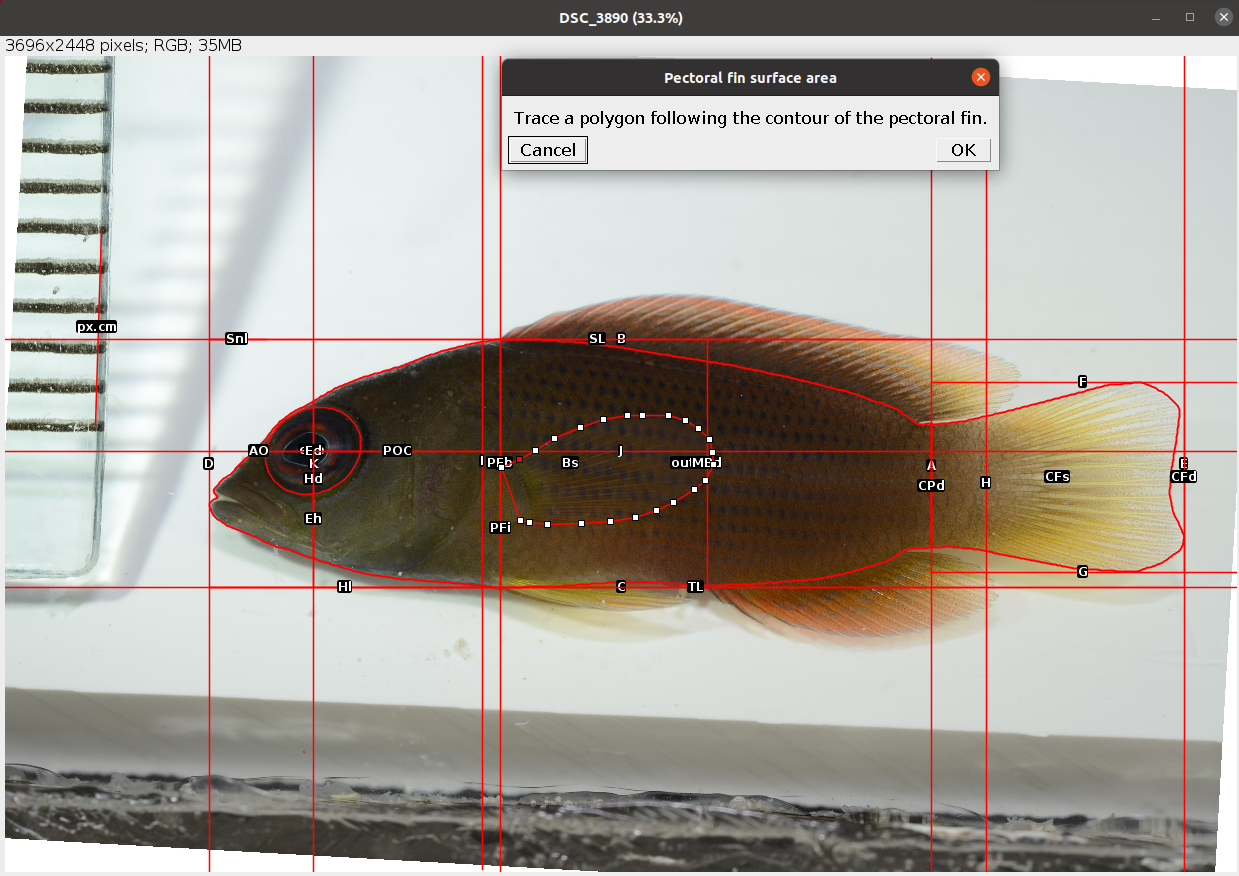
\includegraphics[width=0.8\textwidth,height=\textheight]{./images/screenshots/pectoral_fin_outline.png}

}

\end{figure}

\begin{enumerate}
\def\labelenumi{\arabic{enumi}.}
\setcounter{enumi}{10}
\tightlist
\item
  Trace a line on the longest ray of the pectoral fin. After clicking
  \texttt{OK} this is saved in the ROI manager as PFl.
\end{enumerate}

\begin{figure}

{\centering 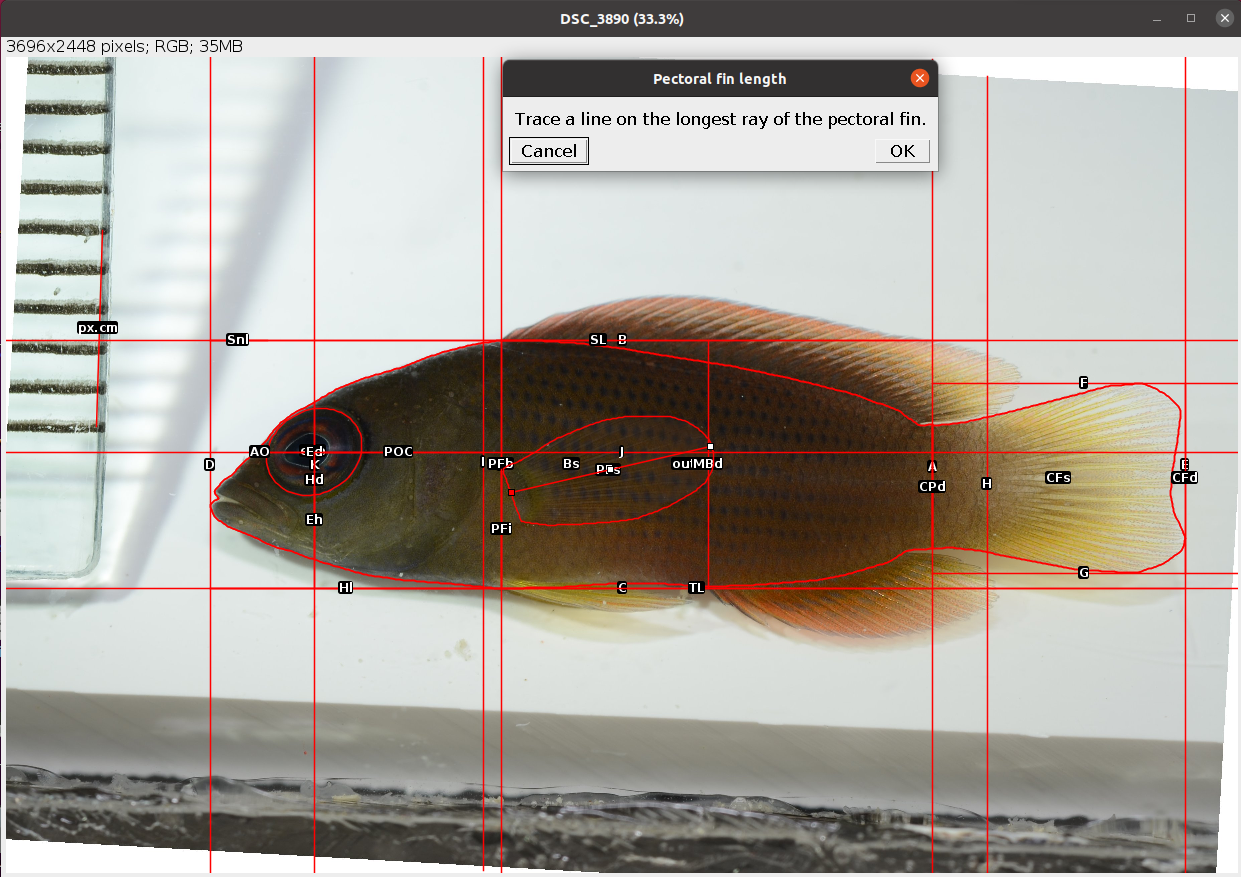
\includegraphics[width=0.8\textwidth,height=\textheight]{./images/screenshots/pectoral_fin_length.png}

}

\end{figure}

\begin{enumerate}
\def\labelenumi{\arabic{enumi}.}
\setcounter{enumi}{11}
\tightlist
\item
  Place a point at the tip of the premaxilla (upper jaw) as in the
  example below. After clicking \texttt{OK} a new trait (Mo) is drawn
  and saved in the ROI manager.
\end{enumerate}

\begin{figure}

{\centering 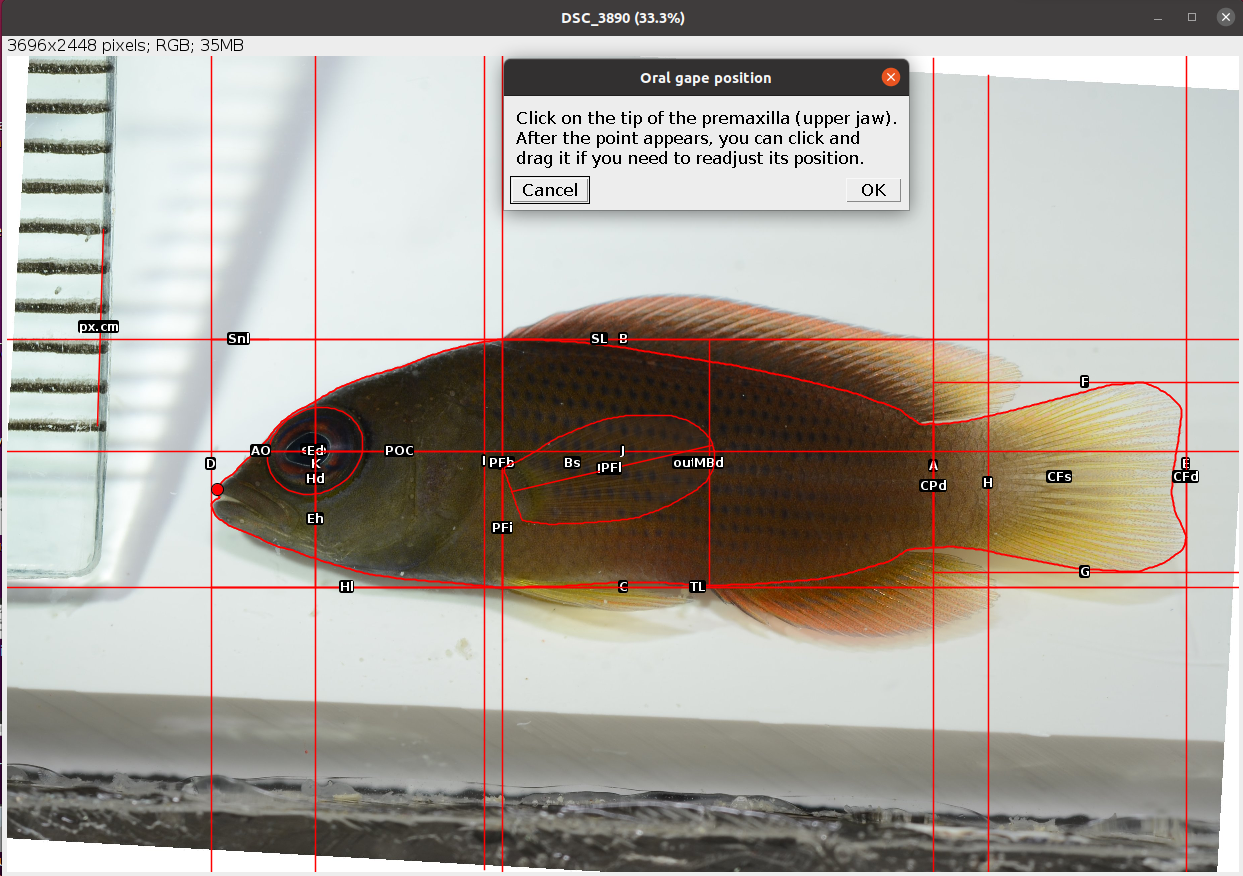
\includegraphics[width=0.8\textwidth,height=\textheight]{./images/screenshots/tip_upper_jaw.png}

}

\end{figure}

\begin{enumerate}
\def\labelenumi{\arabic{enumi}.}
\setcounter{enumi}{12}
\tightlist
\item
  Place a point at the corner of the mouth.
\end{enumerate}

\begin{tcolorbox}[standard jigsaw,arc=.35mm, toptitle=1mm, titlerule=0mm, bottomtitle=1mm, left=2mm, colbacktitle=quarto-callout-important-color!10!white, colback=white, opacityback=0, leftrule=.75mm, title=\textcolor{quarto-callout-important-color}{\faExclamation}\hspace{0.5em}{Important}, coltitle=black, rightrule=.15mm, bottomrule=.15mm, toprule=.15mm, opacitybacktitle=0.6, colframe=quarto-callout-important-color-frame]
The point should be placed at the intersection between the maxilla and
the lower jaw
(\href{https://en.wikipedia.org/wiki/Fish_jaw\#/media/File:FishKeyDay.jpg}{fish
skull anatomy}), not where the flesh of the upper and lower jaw meet!
See the example below.
\end{tcolorbox}

\hypertarget{correct}{%
\subsubsection{\texorpdfstring{\textbf{Correct}}{Correct}}\label{correct}}

\begin{figure}

{\centering 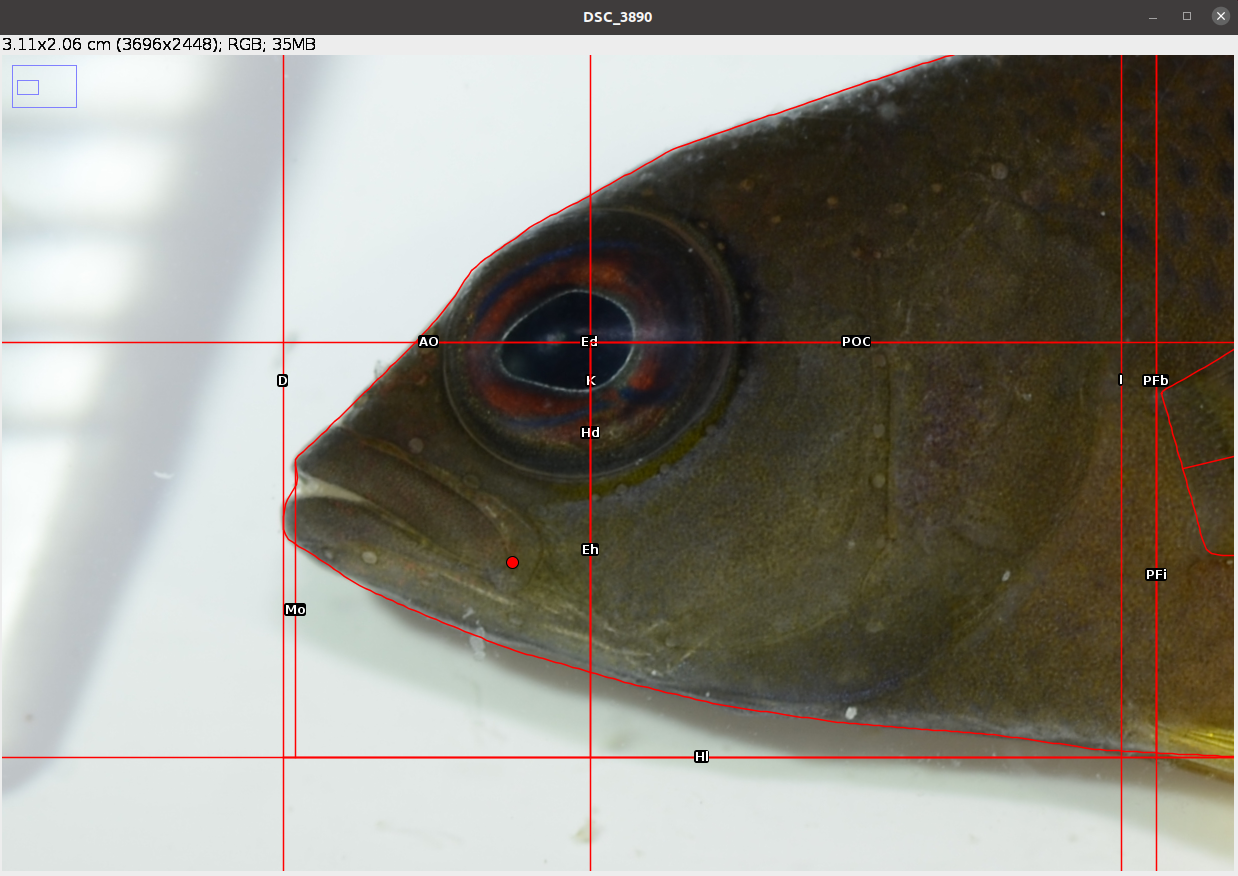
\includegraphics{./images/screenshots/mouth_corner_correct.png}

}

\end{figure}

\hypertarget{incorrect}{%
\subsubsection{\texorpdfstring{\textbf{Incorrect}}{Incorrect}}\label{incorrect}}

\begin{figure}

{\centering 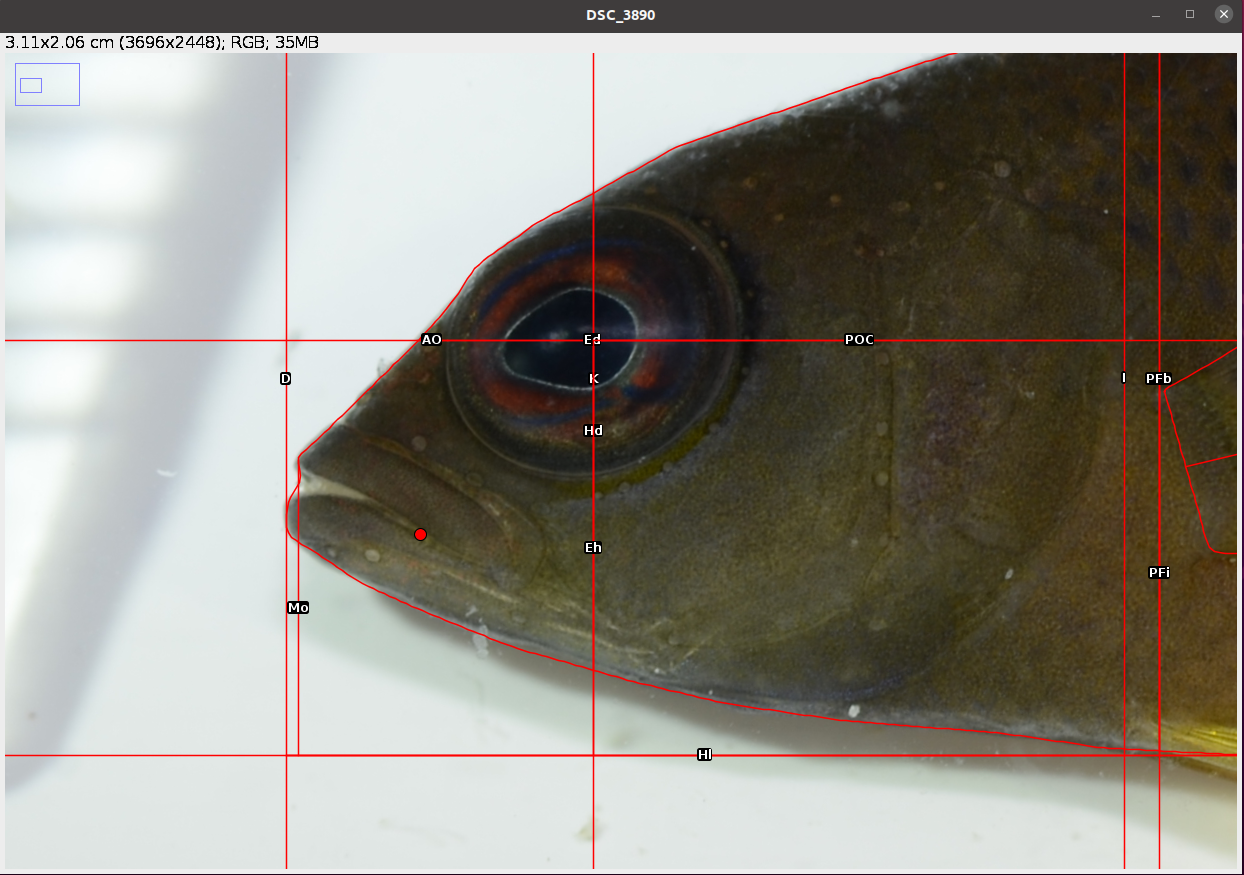
\includegraphics{./images/screenshots/mouth_corner_wrong.png}

}

\end{figure}

After clicking \texttt{OK} the last three traits are drawn and saved in
the ROI manager.

The analysis of the image is completed. In case of single image analysis
a window named \texttt{Traits} containing all the results appears. This
can be saved by clicking on \texttt{File\ -\textgreater{}\ Save\ As...}.
All ROIs in the ROI manager can also be saved as a zip file by clicking
on
\texttt{More\ \textgreater{}\textgreater{}\textgreater{}\ -\textgreater{}\ Save...}.
In case of multiple image analysis a new row will be added to the
results file, the ROIs are saved in their directory, where also the
rotated or straightened images are saved as \texttt{.jpg} files. The
current image is closed and the next is opened. Repeat steps 1-13 for
all images.

\hypertarget{results}{%
\section{Results}\label{results}}

The results file/table contains one row for each image and 25 columns.
The first column, \texttt{image\_id}, is the name of the image without
extension. The second column, \texttt{px.cm}, is the scale of the image
in pixels/cm. The columns 3-24 are the morphometric measurements
described in Table~\ref{tbl-main-traits-def}. Currently, all linear
measurements are in centimetres and all areas in squared centimetres.
The last column, \texttt{time}, is the time spent to analyse the image
(steps 1-13) in seconds.

\hypertarget{sec-head_angles}{%
\chapter{Head Angles}\label{sec-head_angles}}

The \texttt{Head\ Angles} analysis allows to extract three angles
(Figure~\ref{fig-head-angles}, Table~\ref{tbl-angles-def}) related to
vision and feeding (Brandl and Bellwood 2013; Bellwood et al. 2014;
Brandl, Robbins, and Bellwood 2015) from the coordinates of some
reference lines and points (Figure~\ref{fig-angles-ref-lines},
Table~\ref{tbl-angles-ref-lines}).

\begin{figure}

{\centering 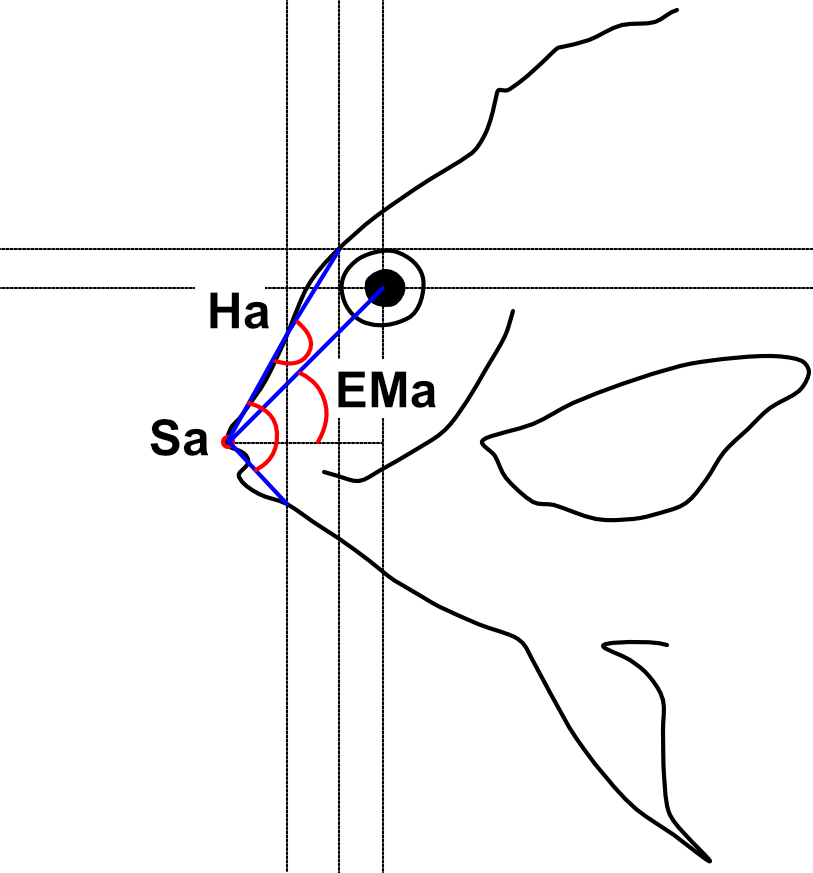
\includegraphics[width=0.5\textwidth,height=\textheight]{./images/drawings/head_angles_sketch.png}

}

\caption{\label{fig-head-angles}Angles measured on fish head (see
Table~\ref{tbl-angles-def} for descriptions)}

\end{figure}

\begin{figure*}

\hypertarget{tbl-angles-def}{}
\begin{longtable}[]{@{}
  >{\raggedright\arraybackslash}p{(\columnwidth - 6\tabcolsep) * \real{0.2027}}
  >{\raggedright\arraybackslash}p{(\columnwidth - 6\tabcolsep) * \real{0.2027}}
  >{\raggedright\arraybackslash}p{(\columnwidth - 6\tabcolsep) * \real{0.3919}}
  >{\raggedright\arraybackslash}p{(\columnwidth - 6\tabcolsep) * \real{0.2027}}@{}}
\caption{\label{tbl-angles-def}Angles measured on fish
head}\tabularnewline
\toprule()
\begin{minipage}[b]{\linewidth}\raggedright
Code
\end{minipage} & \begin{minipage}[b]{\linewidth}\raggedright
Trait
\end{minipage} & \begin{minipage}[b]{\linewidth}\raggedright
Description
\end{minipage} & \begin{minipage}[b]{\linewidth}\raggedright
Reference
\end{minipage} \\
\midrule()
\endfirsthead
\toprule()
\begin{minipage}[b]{\linewidth}\raggedright
Code
\end{minipage} & \begin{minipage}[b]{\linewidth}\raggedright
Trait
\end{minipage} & \begin{minipage}[b]{\linewidth}\raggedright
Description
\end{minipage} & \begin{minipage}[b]{\linewidth}\raggedright
Reference
\end{minipage} \\
\midrule()
\endhead
Ha & Head angle & The angle formed by a line connecting the tip of the
premaxilla (P1) to the point where line L5 crosses the upper margin of
the snout and a line connecting the latter point to the intersection
between lines L3 and L4 & Brandl and Bellwood (2013) \\
Sa & Snout angle & The angle formed by the two lines drawn to the tip of
the premaxilla (P1) from the point where line L5 crosses the upper and
lower margins of the snout & Brandl and Bellwood (2013) \\
EMa & Eye-mouth angle & The angle formed by a line connecting the tip of
the premaxilla (P1) to the eye centroid and a horizontal line
intersecting P1 & Bellwood et al. (2014) \\
\bottomrule()
\end{longtable}

\end{figure*}

\begin{figure}

{\centering 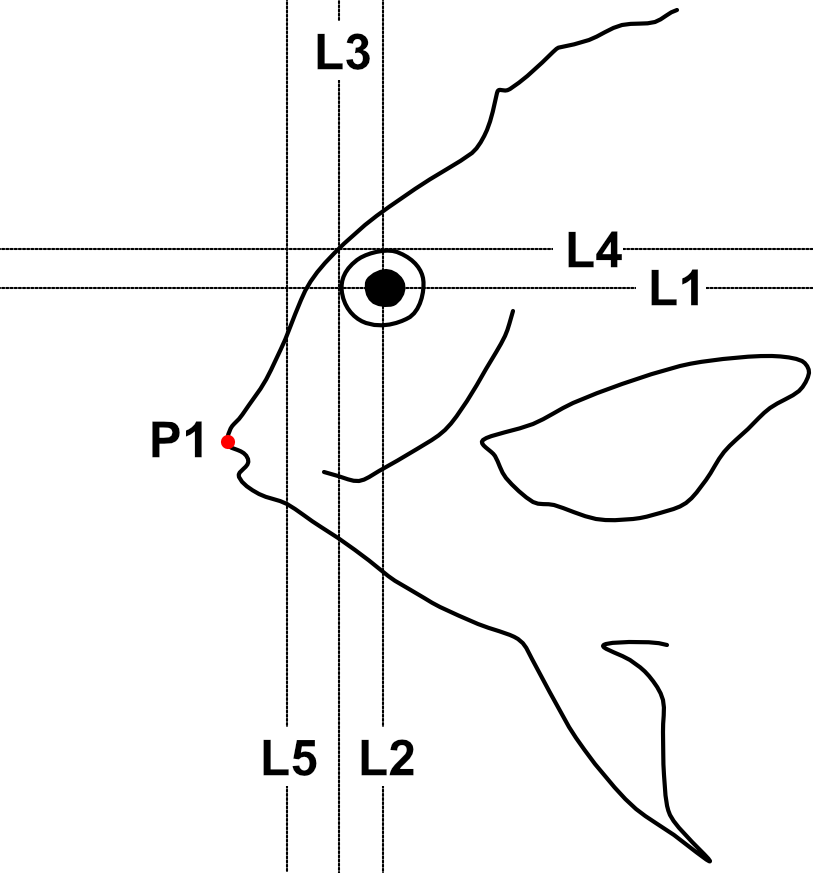
\includegraphics[width=0.5\textwidth,height=\textheight]{./images/drawings/head_ref_lines_sketch.png}

}

\caption{\label{fig-angles-ref-lines}Reference lines and points traced
on fish images for head angles analysis (see
Table~\ref{tbl-angles-ref-lines} for descriptions)}

\end{figure}

\begin{figure*}

\hypertarget{tbl-angles-ref-lines}{}
\begin{longtable}[]{@{}
  >{\raggedright\arraybackslash}p{(\columnwidth - 4\tabcolsep) * \real{0.1781}}
  >{\raggedright\arraybackslash}p{(\columnwidth - 4\tabcolsep) * \real{0.6438}}
  >{\raggedright\arraybackslash}p{(\columnwidth - 4\tabcolsep) * \real{0.1781}}@{}}
\caption{\label{tbl-angles-ref-lines}Description of reference lines and
points traced on fish images for head angles analysis}\tabularnewline
\toprule()
\begin{minipage}[b]{\linewidth}\raggedright
Reference line/point
\end{minipage} & \begin{minipage}[b]{\linewidth}\raggedright
Description
\end{minipage} & \begin{minipage}[b]{\linewidth}\raggedright
User input
\end{minipage} \\
\midrule()
\endfirsthead
\toprule()
\begin{minipage}[b]{\linewidth}\raggedright
Reference line/point
\end{minipage} & \begin{minipage}[b]{\linewidth}\raggedright
Description
\end{minipage} & \begin{minipage}[b]{\linewidth}\raggedright
User input
\end{minipage} \\
\midrule()
\endhead
P1 & Anterior tip of the premaxilla (upper jaw) & Yes \\
L1 & Horizontal line cutting the eye in halves & No\footnote{The user
  needs to trace an ellipse around the eye and lines L1-L4 can be
  automatically drawn from the coordinates of this selection.} \\
L2 & Vertical line cutting the eye in halves & No \\
L3 & Vertical line touching the anterior margin of the eye & No \\
L4 & Horizontal line touching the upper margin of the eye & No \\
L5 & Vertical line half way between L3 and P1 & No \\
\bottomrule()
\end{longtable}

\end{figure*}

\hypertarget{analysis-1}{%
\section{Analysis}\label{analysis-1}}

Once the steps described in Section~\ref{sec-setup} are completed the
screen will be populated with a number of windows:

\begin{itemize}
\tightlist
\item
  the ImageJ/Fiji main window
\item
  the MorFishJ GUI
\item
  a fish image (this is a duplicate of the raw image to prevent any
  modification)
\item
  the ROI manager
\item
  the \texttt{Image\ adjustment} dialog
\end{itemize}

This analysis has six steps that require the user input:

\begin{enumerate}
\def\labelenumi{\arabic{enumi}.}
\item
  Adjust the image if necessary as described in
  Chapter~\ref{sec-straighten_rotate}.
\item
  Select the orientation of the fish (i.e., whether the fish is facing
  left or right) from a drop-down list. This step is important for the
  correct automatic placement of the reference lines.
\end{enumerate}

\begin{figure}

{\centering 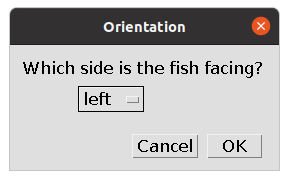
\includegraphics[width=0.3\textwidth,height=\textheight]{./images/screenshots/orientation.png}

}

\end{figure}

\begin{enumerate}
\def\labelenumi{\arabic{enumi}.}
\setcounter{enumi}{2}
\tightlist
\item
  Place a point at the tip of the premaxilla (upper jaw) as shown below.
  After clicking \texttt{OK} this is saved in the ROI manager as P1.
\end{enumerate}

\begin{figure}

{\centering 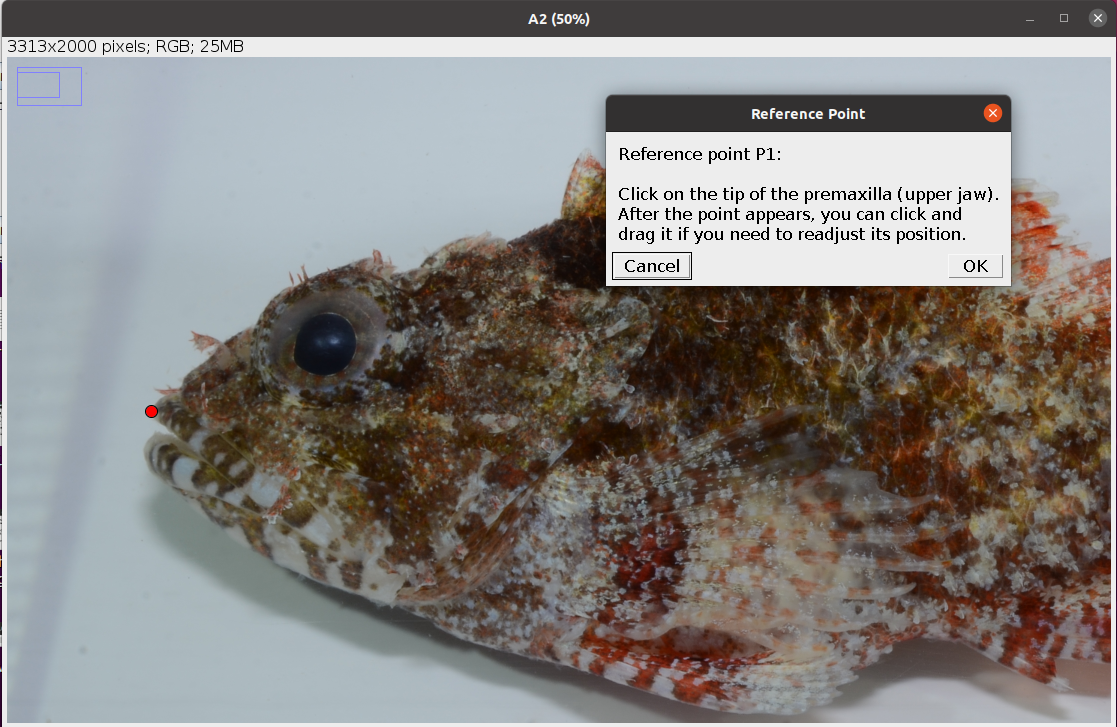
\includegraphics[width=0.8\textwidth,height=\textheight]{./images/screenshots/tip_upper_jaw_head.png}

}

\end{figure}

\begin{enumerate}
\def\labelenumi{\arabic{enumi}.}
\setcounter{enumi}{3}
\tightlist
\item
  Trace an ellipse around the eye as shown below (see
  \href{https://imagej.nih.gov/ij/docs/guide/146-19.html}{Elliptical
  Selection Tool} for specific instructions on how to use this tool).
  After clicking \texttt{OK} five reference lines (L1-L5) are drawn.
\end{enumerate}

\begin{figure}

{\centering 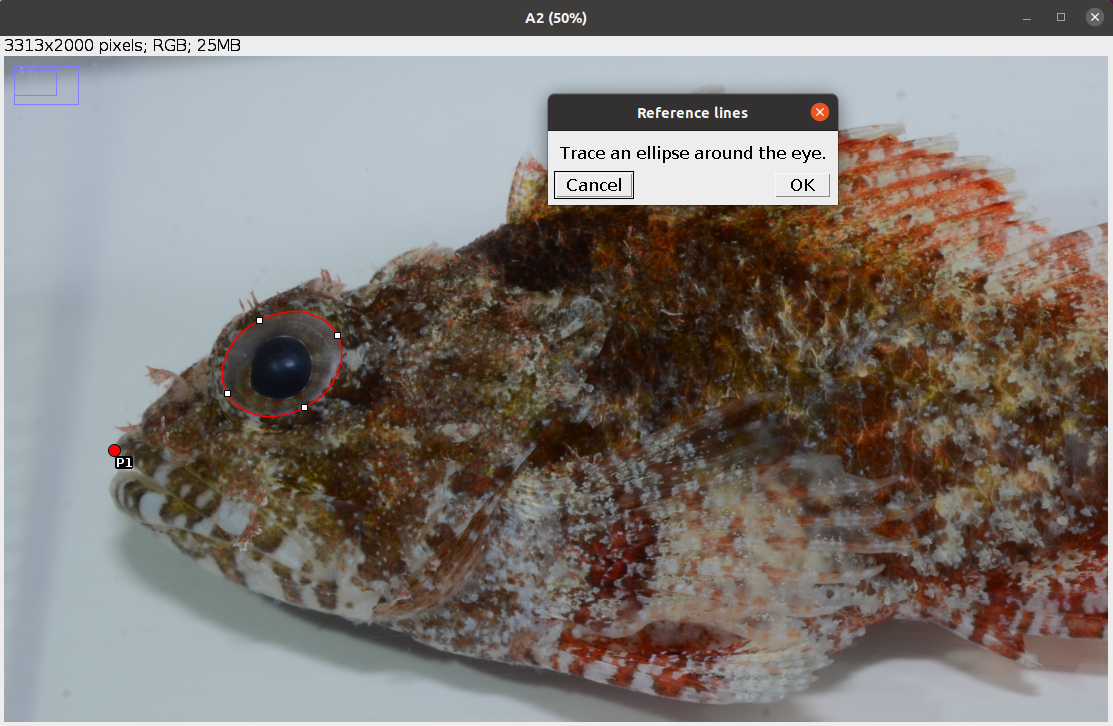
\includegraphics[width=0.8\textwidth,height=\textheight]{./images/screenshots/eye_ellipse_head.png}

}

\end{figure}

\begin{enumerate}
\def\labelenumi{\arabic{enumi}.}
\setcounter{enumi}{4}
\tightlist
\item
  Place a point at the intersection between line L5 and the dorsal
  margin of the snout as shown below. After clicking \texttt{OK} the
  first angle (Ha) is drawn and saved in the ROI manager.
\end{enumerate}

\begin{figure}

{\centering 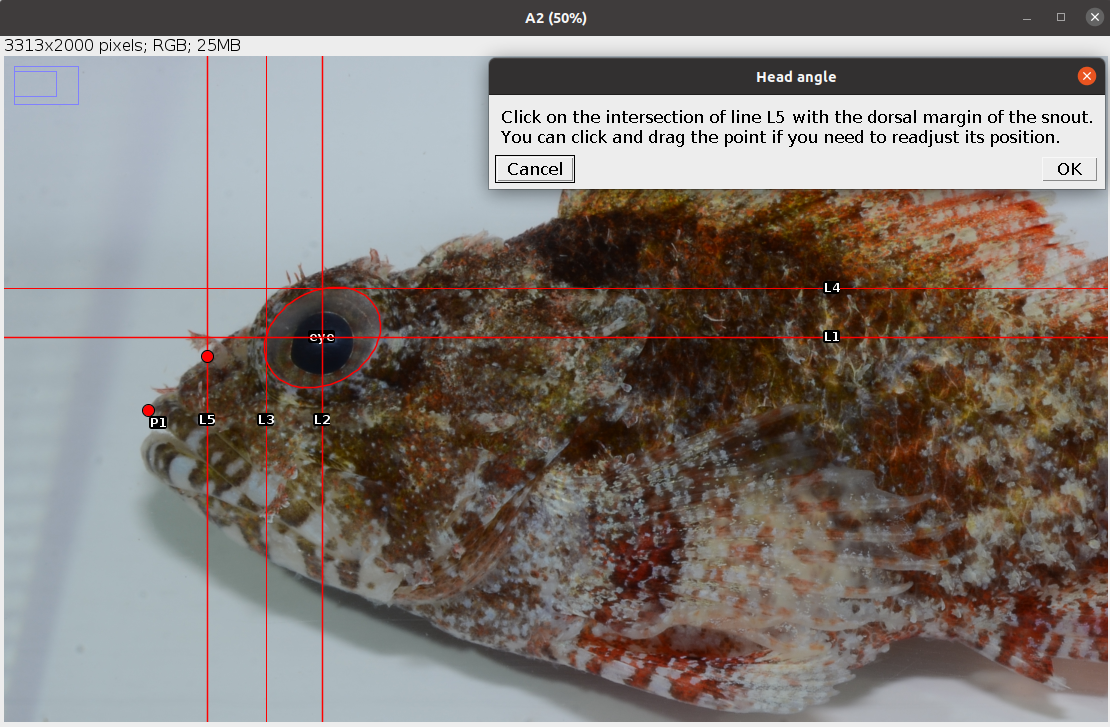
\includegraphics[width=0.8\textwidth,height=\textheight]{./images/screenshots/upper_L5_head.png}

}

\end{figure}

\begin{enumerate}
\def\labelenumi{\arabic{enumi}.}
\setcounter{enumi}{5}
\tightlist
\item
  Place a point at the intersection between line L5 and the ventral
  margin of the snout as shown below. After clicking \texttt{OK} the
  other two angles (Sa, EMa) are drawn and saved in the ROI manager.
\end{enumerate}

\begin{figure}

{\centering 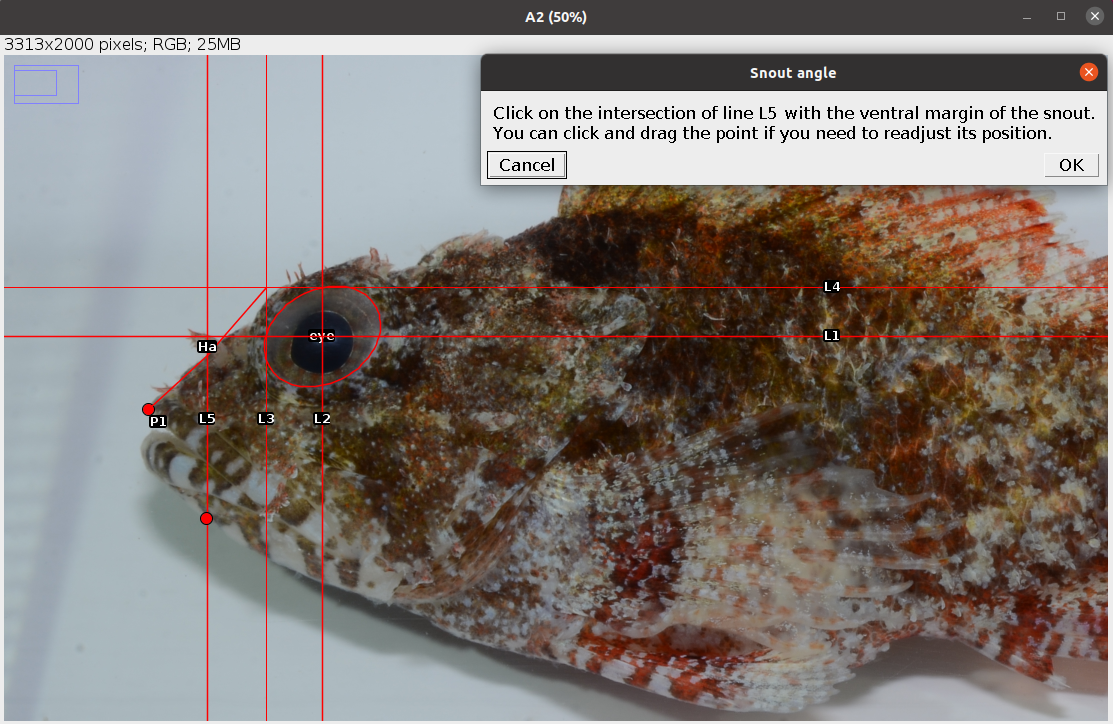
\includegraphics[width=0.8\textwidth,height=\textheight]{./images/screenshots/lower_L5_head.png}

}

\end{figure}

The analysis of the image is completed. In case of single image analysis
a window named \texttt{Traits} containing all the results appears. This
can be saved by clicking on \texttt{File\ -\textgreater{}\ Save\ As...}.
All ROIs in the ROI manager can also be saved as a zip file by clicking
on
\texttt{More\ \textgreater{}\textgreater{}\textgreater{}\ -\textgreater{}\ Save...}.
In case of multiple image analysis a new row will be added to the
results file, the ROIs are saved in their directory, where also the
rotated or straightened images are saved as \texttt{.jpg} files. The
current image is closed and the next is opened. Repeat steps 1-6 for all
images.

\hypertarget{results-1}{%
\section{Results}\label{results-1}}

The results file/table contains one row for each image and 5 columns.
The first column, \texttt{image\_id}, is the name of the image without
extension. The columns 2-4 are the angles described in
Table~\ref{tbl-angles-def} in degrees. The last column, \texttt{time},
is the time spent to analyse the image (steps 1-6) in seconds.

\hypertarget{references}{%
\chapter*{References}\label{references}}
\addcontentsline{toc}{chapter}{References}

\hypertarget{refs}{}
\begin{CSLReferences}{1}{0}
\leavevmode\vadjust pre{\hypertarget{ref-Barnett2006}{}}%
Barnett, A., D. R. Bellwood, and A. S. Hoey. 2006. {``Trophic
Ecomorphology of Cardinalfish.''} \emph{Marine Ecology Progress Series}
322: 249--57. \url{https://doi.org/10.3354/meps322249}.

\leavevmode\vadjust pre{\hypertarget{ref-Bellwood2014}{}}%
Bellwood, D. R., C. H. R. Goatley, S. J. Brandl, and O. Bellwood. 2014.
{``{Fifty million years of herbivory on coral reefs: fossils, fish and
functional innovations}.''} \emph{Proceedings of the Royal Society B:
Biological Sciences} 281 (1781): 20133046.
\url{https://doi.org/10.1098/rspb.2013.3046}.

\leavevmode\vadjust pre{\hypertarget{ref-Brandl2013}{}}%
Brandl, S. J., and D. R. Bellwood. 2013. {``{Morphology, sociality, and
ecology: can morphology predict pairing behavior in coral reef
fishes?}''} \emph{Coral Reefs} 32 (3): 835--46.
\url{https://doi.org/10.1007/s00338-013-1042-0}.

\leavevmode\vadjust pre{\hypertarget{ref-Brandl2015}{}}%
Brandl, S. J., W. D. Robbins, and D. R. Bellwood. 2015. {``{Exploring
the nature of ecological specialization in a coral reef fish community:
morphology, diet and foraging microhabitat use}.''} \emph{Proceedings of
the Royal Society B: Biological Sciences} 282 (1815): 20151147.
\url{https://doi.org/10.1098/rspb.2015.1147}.

\leavevmode\vadjust pre{\hypertarget{ref-Ghilardi2021}{}}%
Ghilardi, M., N. M. D. Schiettekatte, J. M. Casey, S. J. Brandl, S.
Degregori, A. Mercière, F. Morat, Y. Letourneur, S. Bejarano, and V.
Parravicini. 2021. {``{Phylogeny, body morphology, and trophic level
shape intestinal traits in coral reef fishes}.''} \emph{Ecology and
Evolution} 11 (19): 13218--31. \url{https://doi.org/10.1002/ece3.8045}.

\leavevmode\vadjust pre{\hypertarget{ref-Touissant2016}{}}%
Toussaint, A., N. Charpin, S. Brosse, and S. Villéger. 2016. {``Global
Functional Diversity of Freshwater Fish Is Concentrated in the
Neotropics While Functional Vulnerability Is Widespread.''}
\emph{Scientific Reports} 6: 22125.
\url{https://doi.org/10.1038/srep22125}.

\leavevmode\vadjust pre{\hypertarget{ref-Villeger2010}{}}%
Villéger, S., J. R. Miranda, D. F. Hernández, and D. Mouillot. 2010.
{``Contrasting Changes in Taxonomic Vs. Functional Diversity of Tropical
Fish Communities After Habitat Degradation.''} \emph{Ecological
Applications} 20 (6): 1512--22. \url{https://doi.org/10.1890/09-1310.1}.

\end{CSLReferences}



\end{document}
